\documentclass[a4paper,11pt]{article}

%
% Do not change
\textheight = 220mm
\textwidth = 150mm
\topmargin = 10mm
\oddsidemargin = 5.0mm
\evensidemargin = 5.0mm
\unitlength = 1mm


\usepackage[T1]{fontenc} % Use latin1 font encoding

\usepackage[UKenglish]{babel}

\usepackage{csquotes} % For blockquote
\usepackage{enumitem}

\usepackage{caption}
\usepackage{subcaption}

\usepackage[section]{placeins} % FloatBarrier
\usepackage{graphicx} % Figures
\graphicspath{{./figures/}} % Simplify figure importing
\DeclareGraphicsExtensions{.pdf,.png} % Simplify figure importing

\usepackage{hyperref} % links

% ----- Format code files start
\usepackage{amsmath}
\usepackage{xcolor}
\usepackage{listings}
\lstset{
  basicstyle=\tiny,
  frame=single,
  breaklines=true
}
% ----- Format code files end

\usepackage[final]{pdfpages} % used to include pdf to appendicies

\begin{document}

\let\rempage=\thepage
{
\renewcommand{\thepage}{\relax}
\begin{figure}
	
\includegraphics[width=0.18\textwidth]{mahlogo-name}
\end{figure}

\vspace*{-30mm}
\hfill\begin{minipage}[t]{10em}\large
Teknik och samh�lle\\
Datavetenskap
\end{minipage}

\vspace*{45mm}
\begin{center}
{\bf\large
Examensarbete

\small
15 h�gskolepo�ng, grundniv�
}

\vspace*{25mm}
\LARGE

The differences in requirement elicitation between community- and firm-driven open source software projects on Github. 

\vspace*{8mm}
\large

Examensarbetets titel p� svenska %TODO

\vspace*{12mm}
\Large
%
% Author names
Teddy Andersson\\
Filip Harald

\vspace*{30mm}
\large
% picture TODO?
\end{center}

\vfill
\hspace*{-10mm}%
\begin{minipage}[t]{20em}
%
% Fill in correct data for you
Examen:~kandidatexamen 180~hp
\\
Huvudomr�de:~datavetenskap
\\
Program:~systemutvecklare
\\
Datum f�r slutseminarium:~TBD
\end{minipage}
\hfill
\begin{minipage}[t]{20em}
Handledare: Nancy Russo
\\
Assisterande handledare: Aleksander Fabijan
\\
Examinator:~Carl Magnus Olsson
\end{minipage}

\newpage

\mbox{}

\newpage

\section*{Sammanfattning}

Denna sammanfattning kommer skrivas inf�r slutgiltiga inl�mningen.

\newpage

\mbox{}

\newpage

\section*{Abstract}
Knowledge about the variety of options among project process when starting up a new software development project is crucial for the developers, the governing bodies and the end product. Therefore new and unfamiliar options are taken out of the equation to make sure that the work gets done and that the solution will be delivered on time and with high quality. This behavior in long term does however exclude new and better ways of executing the work in the process. So to shine light upon new development methods and enlighten those who are in need of insight into a new viable option we chose to investigate the differences in requirement elicitation within the area of Open Source Software (OSS) Development. By examine how and by who requirements are elicited in a firm-driven project compared to a community driven project, we framed a total of three research question to base our case study on. The case study showed that in community driven OSS projects external users have a low participation compared to firm-driven projects where the participation is high. Finally we could conclude that firms can reduce their development costs by engaging in OSS development.

%Keywords
\textbf{\textit{Keywords---open source software, development process, requirement elicitation, git, Github, Atom, Neovim}}

\newpage

\mbox{}

\newpage
\tableofcontents
\newpage
\ifodd\value{page}\else\mbox{}\newpage\fi
\setcounter{page}{1}
\renewcommand{\thepage}{\rempage}

\section{Introduction}
\label{sec:intro}

%Problem and challenges
Today we are constantly introduced to new software applications and systems that we install on our smartphones, tablets and computers. Behind each software that we choose to install and use on our devices is a development process with several defined steps to be completed before we can put our hands on the software and try it out. The steps that takes a software from an idea to a final product are many and the different methods to solve this process are often hard to choose for those who are set to develop the software. Choosing a method to follow throughout this process are therefore important in the aspects of expenses, time and software quality. Despite the choice of method there will always be an constant work to understand the user needs, from the needs necessary functionality can be written down in paragraphs, in the area of computer science we call these paragraphs requirements, so the software developers know what to implement into the software during the process. The elicitation of these requirements in a development process based on a Open Source Software(OSS) development method, a development method where the source code of a software is available and open to anyone, are faced by several challenges. First, Curtis et al \cite{Curtis1986} explain in 1986 that software development is a knowledge-intensive activity with a large number of potentially confounding factors, in 2016 Minghui et al. \cite{Zhou2016} further explained that this makes it difficult or impossible to discern the impact of commercial involvement from different types of companies. Second, Minghui et al. \cite{Zhou2016} continues to explain that to observe the impact of commercial involvement, it is important to compare the differences in contributions from developers, and to observe the work impact on projects over a long period of time. Third, there is no easy way to learn companies', intentions motivating their involvement in the Open Source Software (OSS) community, and it is even more difficult to examine the effects of such involvement.

%Problem and challenges(Old introduction): Today there are several methods to choose from when you decide to develop or continue the integration of software, and every method has its own benefits and fits some software projects better than others. While deciding which method to choose there are always a variety of factors that must be taken into consideration. One of these factors is elicitation of the requirements, paragraphs that explain a functional or nonfunctional feature requirement that the software must be able to handle. In a development project, this factor is effected by several challenges. First, software development is a knowledge-intensive activity with a large number of potentially confounding factors~\cite{Curtis1986}, and this makes it difficult or impossible to discern the impact of commercial involvement. Second, to observe the impact of commercial involvement, it is important to compare the differences in contributions from developers, and to observe the work impact on projects over a long period of time. Third, there is no easy way to learn companies', intentions motivating their involvement in the Open Source Software (OSS) community, and it is even more difficult to examine the effects of such involvement.

%Purpose
The challenges described above are key factors for this thesis purpose, to enlighten the decision of developing software with an open source software (OSS) development approach. By providing this information of governing bodies, regardless if there is a firm or a community managing the project, the initial decision of choosing a software development approach could be made easier. This thesis will however not make a comparison between open source and proprietary software. Therefore this thesis will also not provide pros and cons of the transition from proprietary software to OSS. Bottom line, the thesis will help governing bodies realise that OSS truly can deliver quality software, enthusiastic developers, better costumer relationships and commercial available software.

%Contribution
As a result of this study we will have made the following three contributions. (a) When studying the characteristics of two OSS-projects the results will of course contribute to the general knowledge about OSS development. (b) As mentioned above our results can be used as support for a firm when deciding if they want to use OSS development. (c) The scripts we have programmed and used to process the project artefacts of the two projects. These scripts are modular and can be used to retrieve information about a large group of open source projects.

%Approach
This thesis presents a comparative case study of differences and commonalities in requirement elicitation between firm-driven and community-driven OSS projects on Github: Atom and Neovim. We address key questions about their differences towards each other overall and within the area of requirement elicitation, based on data gathered from Github. Based on the work of~\cite{Mockus2002a} and~\cite{Noll} we framed a number of hypotheses that we conjectured would be true generally for both development and requirement elicitation within the area of OSS-development.

\subsection{Background}
\label{subsec:background}

\begin{displayquote}
	\textit{"A great babbling bazaar of differing agendas and approaches out of which a coherent and stable system could seemingly emerge only by a succession of miracles."}~\cite{catb}
\end{displayquote}

%introduce the reader to the section
	%Introduce the reader to System Development
In the evolution of software development different types of methods have been used to manage initiation, planning, execution, monitoring and closeout of a software project. The project methods which where first to adopt these phases are known as traditional development methods. The traditional development approach identifies a sequence of steps to be completed, where the work of a new step doesn't begin until the previous step is completed. However methods were not optimal for software development, where the need for continuos integration is important~\cite{Jansson2015}. Therefore on February 11, 2001, at The Lodge at Snowbird ski resort in the Wasatch mountains of Utah, 17 people met to talk, ski, relax and try to find common ground~\cite{Fowler2001}. What emerged under this meeting was the Agile Software Development Alliance. From this alliance the Agile methods evolved based on a manifesto where the effort was to overcome perceived and actual weakness in conventional software engineering~\cite{Fowler2001}. This alliance wrote down the famous Agile Manifesto and their reason was simply to uncover better ways of developing software by doing it and helping others do it~\cite{Fowler2001}. In contrast to the traditional methods the agile methods are based on incremental methods, managing the design and build activities of engineering~\cite{Jansson2015}. Apart from the traditional and agile methods the open source software (OSS) development method started to received a lot of attention in the late 90's. OSS development is the process by which open-source, or similar software whose source code is publicly available, is developed. These are software products available with its source code under an open-source license to study, change and improve its design. For this reason OSS was in the late 90's characterised as a fundamental new way to develop software and was seen as a challenge to the commercial software business that dominated the vast majority of the software market~\cite{Mockus2002a}. Over time, OSS evolved into a method that can be applied on commercial software and maintain quality. Examples of some popular open-source software products are Mozilla Firefox, Google Chromium, Android, Linux, the Apache OpenOffice Suite, Atom and Neovim. Open-source software development has been a large part of the creation of the World Wide Web as we know it, with Tim Berners-Lee contributing his HTML code development as the original platform upon which the internet is now built~\cite{timbernerslee}.

	%TODO: More on the open source story

	%Introduce the reader to Community-driven projects and Requierment elicitaton
Regardless of the development process a project chooses to use when developing a software system they would most likely need a way to handle requirements in one way or another. While requirements in traditional and agile development processes are elicited from discussions with a client/customer OSS project handles the elicitation through the users/developers that are involved in the OSS community. People in these communities cooperate via the Internet and never, or seldom, meet face to face. The number of developers can differ from a handful to thousands and are often geographically distributed~\cite{Maccormack2006}. Joblin et al.~\cite{joblin} describes the two vital roles of developers in a OSS project, where they so called core developers are developers with a substantial, long-term involvement, and in a abstract sense these developers plays an essential role in developing the system architecture and forming the general leadership structure. In contrast, peripheral developers are typically involved in bug fixes or small enhancements, and they they have irregular or short-term involvement. 

%The key decisions in project driven by OSS communities are taken by a central group of software developers (core developers). Beyond this central group, are the peripheral developers; these are developers who intermittently submit code contributions (called patches). The core group reviews and acknowledge the patches before they are incorporated into the projects source code~\cite{Crowston2006}. 

%Introduce the reader to Firm-driven development
The Agile methods are popular to use in software companies for information systems development. Agile methods are claimed to encourage developers to be more flexible and efficient by means of arrangements in the development teams physical and social environment~\cite{Jansson2015}. In recent years, however, we have seen an increased interest in using open source alongside with the Agile development~\cite{Author2008,Jansson2015}. Large-scale companies like Google, Microsoft, Facebook etc have been striving towards a more open environment in both development projects but also in general work process~\cite{Schmidt2014}. Alongside with an interest and momentum of OSS it is now also considered to be, in a commercial settings, a more viable approach~\cite{Author2008}. From a commercial stand point OSS development also promises many advantages. Including reduced salary costs; reduced cycle time arising from' 'follow-the-sun'' software development; cross-site modularisation of development work; access to a larger skilled developer pool; innovation and shared best practice; and closer proximity to customers~\cite{Author2008}.

\subsection{Related Work}
\label{related_work}
%Explain the context of the other two studies and their findings/limitations

% apache and mozilla
In previous work within the area of OSS and requirement elicitation there are two highly relevant studies for this thesis. The first article~\cite{Mockus2002a} presents two case studies of the development and maintenance of major OSS projects: the Apache server and Mozilla. Where Mockus et al. address key questions about the development process, and about the software that is the result of the processes. Based on results from a earlier study made on Apache, covered in the article A Case Study of Open Source software Development: the Apache server, they framed a number of hypotheses that they conjectured would be true generally of open source developments. The second case study in the article~\cite{Mockus2002a} examined data from the Mozilla project based on the analyses and hypothesis that were framed from the Apache project. Mockus et al. came to the conclusion that the essential differences in which elements of commercial and open source processes coordinate, select, and assign work could be combined. To make their generalisation trustworthy they selected the two cases which can be considered typical instances for an OSS-project, Apache and Mozilla. The authors present 6 research questions for which they motivate should be sufficient to compare with other projects~\cite{Mockus2002a}. The 6 questions are presented in Table~\ref{tab:apache}.

\begin{table}[h]
	\centering
	\begin{tabular}{ | p{0.9\textwidth} |}
		\hline
		\begin{enumerate}
			\item What were the processes used to develop Apache and Mozilla?
			\item How many people wrote code for new functionality? How many people reported problems? How many people repaired defects?
			\item Were these functions carried out by distinct groups of people, that is, did people primarily assume a single role? Did large numbers of people participate somewhat equally in these activities, or did a small number of people do most of the work?
			\item Where did the code contributors work in the code? Was strict code ownership enforced on a file or module level?
			\item What is the defect density of Apache and Mozilla code?
			\item How long did it take to resolve problems? Were high priority problems resolved faster than low priority problems? Has resolution interval 	decreased over time?
		\end{enumerate}\\
		\hline
	\end{tabular}
	\caption{Research questions for exploring OSS-projects~\cite{Mockus2002a}.}
	\label{tab:apache}
\end{table}

\FloatBarrier

% firefox and openemr (req. elicitation) 
In the second highly relevant article,~\cite{Noll}, Noll et al. presents a case study of the OpenEMR, an open source project developing electronic medical record (EMR) software. The goal of the study was to understand how requirements are elicited, documented, agreed and validated in a small open source software project. The study followed the same approach as of an earlier study of the Firefox web browser~\cite{Noll2008a}. The comparison between the both projects showed that, similar to the Firefox study, the majority of OpenEMR requirements are asserted by developers. Documentation was informal, consisting mainly of archived discussions. Contributors to the OpenEMR project were medical practitioners such as doctors or clinic administrations, who use the product in their practices and also developers which does not use the product at all. The implication for software development in general is that developers can be a significant source of innovation. In order to conduct the study the authors present a method including 5 steps for retrieving the data upon which they will make the comparison. The method is presented in Table~\ref{tab:openemr}.

% firefox and openemr (req. elicitation) 
\begin{table}[h]
	\centering
	\begin{tabular}{ | p{0.9\textwidth} |}
		\hline
		\begin{enumerate}
			\item Identify the set of features delivered for OpenEMR after release 2.8.0, up to and including release 2.9.0.
			\item Select a subset of these features for examination.
			\item Examine Internet resources related to OpenEMR, such as archives of discussion forums, the OpenEMR issue database, the OpenEMR ''tracker'' on Sourceforge.net, and other online forums, to discover when the feature was first proposed, and what role the person proposing the feature played (such as user or developer).
			\item Determine the initial implementation of the feature (prototype by a developer, patch submitted to the tracker, or enhancement committed directly to the codebase).
			\item Categorise the requirement as asserted by a developer, either from his or her personal experience or knowledge of user needs; proposed by an end-user, for example by posting a request to one of the discussion forums, or filing a bug report or ''Request for Enhancement'' in the issue database; or derived from features found in competing products.
		\end{enumerate}\\
		\hline
	\end{tabular}
	\caption{5 steps for gathering data from OSS-projects~\cite{Noll}.}
	\label{tab:openemr}
\end{table}

\FloatBarrier

%Communicate to the reader that what WE are doing has not been done just yet.

The articles together summarise the differences between open-source projects in different aspects. Mockus et al.~\cite{Mockus2002a} investigate two cases from which they try to form theories on what it is that defines OSS-projects. They conclude the study by comparing their results with commercial, proprietary, projects. Noll et al.OSS-projects~\cite{Noll} on the other hand investigate the differences in requirement elicitation between large and small OSS-projects. These articles are the two most relevant studies in comparing requirement elicitation in OSS projects due to the contributions in form of methods that can be applied to several aspects in comparing different types of OSS-projects.

\subsubsection{Case Study}
%what is a case study?
Oates refers to a case study as being research strategy for which one tries to describe a case, or phenomenon, from within its natural context~\cite{Oates2005}. Rather than just confirming a phenomenons existence, which could be done by for example conducting a survey, a case study aims to discover why it occurred. This is done, as a researcher, by aiming to give a detailed description of not just the phenomenon but also it's context. It is from the context the researcher can identify factors which might have caused the phenomenon to occur. The amount of factors varies from case to case and the probability of multiple causing factors should be taken into account.

%internet case studies
Oates says that case study can favourably be used when ''studying the 'life' on the Internet''~\cite{Oates2005}. However the author mentions particular issues with conducting this kind of research. The first is the problem of boundary. Namely how does one define the boundaries for which the study is being conducted. The second is the problem of offline/online existence. That is one might not get all the details for a case by only studying it online, since some information might only be available offline, such as communications between participants of the studied case. These problems are taken into consideration when constructing our method for conducting the case study. However, the first problem will have minimal effect on our research since it's easy to define what is part and not of the development process of a product and what is not. The second problem on the other hand could affect our research to greater extent. The nature of OSS is that everything related to the project is stored and displayed online. But even though developers might never meet face-to-face, they may still communicate on other channels than those provided through the project. These channels are not always displayed online and can therefore be seen, from a researchers perspective, as offline.

\subsection{Research Question}
\label{sec:rq}
Based on our research interests in studying the commonalities and differences between community and firm driven OSS projects, we present our research questions below. The first research question (RQ) addresses the characteristics of community-driven OSS development. The second RQ addresses the characteristics of firm-driven OSS development. The third and last RQ addresses the result of what the first two and what they imply.
\begin{enumerate}[label=RQ\arabic*]
	\item \emph{What are the characteristics of community-driven OSS development?}
	\item \emph{What are the characteristics of firm-driven OSS development?}
	\item \emph{What are the implications of the differences between firm- and community-driven OSS development?}
\end{enumerate}

%Shortly describe structure of report
The remainder of this paper is organised as follows: the next section will present our systematic literature review which we conducted to familiarise with the subject; the next section will present the chosen method for this study; next are the results; they are followed by an analysis and discussion of their implications; lastly we present a conclusion and suggestions for future work.
%-----------------------------------------------------------------------------------------------------------------------------------------------------------------------

\newpage
\section{Systematic Literature Review}
To ensure that our thesis is credible we first have to make sure that we are well informed on the subject we're researching. In order to do this we've performed a systematic literature review. which is presented in this section.

When searching we used three different databases: \emph{ACM Digital Library} (\texttt{ACM}), \emph{IEEE Xplore Digital Library} (\texttt{IEEE}) and \emph{Google Scholar} (\texttt{GOOGLE}). The first two, \texttt{ACM} and \texttt{IEEE}, are well-known within the area of computer science and they were used for searching for articles using keywords and search phrases. The last, \texttt{GOOGLE}, was used for forward and backward snowballing.

When searching in \texttt{ACM} and \texttt{IEEE} we used different combinations of keywords and sometimes filters to refine the search. As we read more papers on the subject the list of keywords was extended. We used the following keywords: \emph{''open source'', open, source, success, software, development, community, requirements, corporate, firm, project, ''case study''} and \emph{case, study}. Used search phrases with their results are presented in table~\ref{tab:results}.

\begin{table}[!h]
	\begin{tabular}{ | l | c | c | c |}
		\hline
		\textbf{Search Phrase} 								& \textbf{Filters}			& \textbf{\texttt{ACM}} 	& \textbf{\texttt{IEEE}}	\\\hline
		''open source'' AND success			 				& - 						& 333 				& 330				\\\hline
		''open source'' AND success	 						& only matching in title		& 6 					& 21					\\\hline
		open AND source AND software AND development	 		& - 						& 2618 				& 260				\\\hline
		open AND source AND software AND development	 		& only matching in title		& 99 					& 0					\\\hline
		open AND source AND development AND community	 	& - 						& 1129 				& 684				\\\hline
		open AND source AND development AND community	 	& only matching in title		& 25 					& 0					\\\hline
		open AND source AND development AND requirements	 	& - 						& 734 				& 137				\\\hline
		open AND source AND development AND requirements	 	& only matching in title		& 5 					& 0					\\\hline		
		''open source'' AND corporate AND project		 		& - 						& 1689 				& 28					\\\hline
		''open source'' AND corporate AND project		 		& only matching in title		& 67 					& 0					\\\hline
		''open source'' AND firm AND project				 		& - 						& 20 					& 2264				\\\hline
		''open source'' AND firm AND project				 		& only matching in title		& -					& 45					\\\hline
		''open source'' AND firm AND community				 	& - 						& 14 					& 1412				\\\hline
		''open source'' AND firm AND community				 	& only matching in title		& 0 					& 39					\\\hline
		''open source'' AND corporate AND project AND community	& - 						& 540 				& 0					\\\hline
		''open source'' AND corporate AND project AND community	& only matching in title		& 15 					& 0					\\\hline
		case AND study\footnotemark							& only matching in title		& 384 				& 156				\\\hline
	\end{tabular}
	\caption{Used search phrases and filters and amount of results.}
	\label{tab:results}
\end{table}

\FloatBarrier
\footnotetext{We read through most of these even though they were more than 100}
When the amount of search results were maximum 100 we went through the studies doing the first pass of Keshavs \emph{three-pass approach}~\cite{Deming2010}. If the article was found interesting we added it to our reference manager to later perform the second and third pass on. For each article which after the second pass still was found relevant we noted the references to snowball more articles, this process is described in the next section. 

We used \texttt{GOOGLE} to snowball more studies. This was done in three parts for every study: (1) search for all references used in the study, (2) search for all studies that referenced to the study and (3) search for more studies written by the same author(s). Searches in \texttt{GOOGLE} sometimes generated a huge amount of results and also the results did not always have the article itself available for download. In those cases we used \texttt{ACM} and \texttt{IEEE} to limit the result or find the article. Keshavs \emph{three-pass approach} was also here used for selecting relevant articles~\cite{Deming2010}. All our relevant studies are presented in Table~\ref{tab:relevant}.

\begin{table}
	\resizebox{!}{.35\paperheight}{\begin{tabular}{ p{0.6\textwidth} | p{0.15\textwidth} | p{0.1\textwidth} | p{0.4\textwidth}}
		\hline
		\textbf{Name of Article}	& \textbf{How it was found}	& \textbf{How many articles was snowballed form this}	& \textbf{Used search phrase}\\\hline
		A Case Study of Open Source software Development: the Apache server	& \texttt{ACM} or \texttt{IEEE}	& 1 & open AND source AND software AND development \\\hline
		Agila projektledningsmetoder och motivation & \texttt{GOOGLE}	& 0 & open source + konventionell + project + management + case study \\\hline
		An analysis of requirements evolution in open source projects: recommendations for issue trackers	& \texttt{ACM} or \texttt{IEEE}	& 0 & open AND source AND development AND requirements \\\hline
		Balancing act: community and local requirements in an open source development process	& \texttt{ACM} or \texttt{IEEE}	& 0 & open AND source AND development AND community \\\hline
		Case Study Research: Design and Methods	& Snowballed	& 0 & - \\\hline
		Challenges and recommendations for the design and conduct of global software engineering courses: A systematic review	&  \texttt{ACM} or \texttt{IEEE}	& 0 & ?? \\\hline
		Classifying Developers into Core and Peripheral: An Empirical Study on Count and Network Metrics	& Personal recommendation	& 0 & - \\\hline
		Comparative Case Studies	& Snowballed	& 0 & - \\\hline
		Evolution in open source software: a case study	& \texttt{ACM} or \texttt{IEEE}	& 0 & ?? \\\hline
		Exploring the Structure of Complex Software Designs: An Empirical Study of Open Source and Proprietary Code	& Snowballed	& 2 & - \\\hline
		Free/Libre open-source software development	& \texttt{ACM} or \texttt{IEEE}	& 1 & ''open source'' AND success \\\hline
		From a Firm-Based to a Community-Based Model of Knowledge Creation: The Case of the Linux Kernel Development	& Snowballed	& 0 & - \\\hline
		How Can Open Source Software Development Help Requirements Management Gain the Potential of Open Innovation: An Exploratory Study	& \texttt{ACM} or \texttt{IEEE}	& 0 & open AND source AND development AND requirements \\\hline
		How Google Works	& Snowballed	& 0 & - \\\hline
		Inflow and Retention in OSS Communities with Commercial Involvement	& \texttt{ACM} or \texttt{IEEE}	& 0 & ''open source'' AND corporate AND project AND community \\\hline
		Information systems success in free and open source software development: Theory and measures	& Snowballed	& 0 & - \\\hline
		Innovation Model : Issues for Organization Science Open Source Software and the ''Private-Collective'' Innovation Model : Issues for Organization Science	& Snowballed	& 0 & - \\\hline
		Open Sources: Voices from the Open Source Revolution	& Snowballed	& 0 & - \\\hline
		Peripheral Developer Participation in Open Source Projects	& \texttt{ACM} or \texttt{IEEE}	& 1 & ''open source'' AND corporate AND project \\\hline
		Requirements acquisition in open source development: Firefox 2.0	& Snowballed	& 0 & - \\\hline
		Requirements elicitation in open source software development: a case study	& \texttt{ACM} or \texttt{IEEE}	& 2 & open AND source AND software AND development \\\hline
		Researching information systems and computing	& Course literature from previous course	& 0 & - \\\hline
		Software Psychology: The Need for an Interdisciplinary Program	& Snowballed	& 3 & - \\\hline
		The agile manifesto	& \texttt{GOOGLE}	& 0 & ?? \\\hline
		Two case studies of open source software development: Apache and Mozilla	& Snowballed	& 0 & - \\\hline
		Why do users contribute to firm-hosted user communities? The case of computer-controlled music instruments	& Personal recommendation & 1 & - \\\hline

	\end{tabular}}
	\caption{Shows the names of the articles relevant to our thesis and how they were found.}
	\label{tab:relevant}
\end{table}

\FloatBarrier
Out of the studies presented in Table~\ref{tab:relevant} we currently use seven of them. The studies and how they were found are presented below.

\begin{enumerate}
	\item \textbf{Software Psychology: The Need for an Interdisciplinary Program~\cite{Curtis1986}}
	
	The search phrase \texttt{acmdTItle:(+"open source" +corporate +project +community)} on \texttt{ACM} resulted in 15 hits. One of them was~\cite{Zhou2016} which after the second pass we still found relevant. When going through its references we found the following relevant articles:~\cite{RobertK1994},~\cite{Goodrick2014} and also~\cite{Curtis1986} which is used in our thesis.
	
	\item \textbf{Agila projektledningsmetoder och motivation~\cite{Jansson2015}}
	
	When researching on how we could introduce the reader to agile project management and open source we also used \texttt{GOOGLE} to do some searches in Swedish, our native language. The search phrase \texttt{(''open source'' + konventionell + projektledning + ''case study'')} then resulted in 8 hits. One of the was~\cite{Jansson2015} which we found relevant in the first pass.
	
	\item \textbf{Classifying Developers into Core and Peripheral : An Empirical Study on Count and Network Metrics~\cite{Joblin}}
	
	This article was recommended to us by our supervisor. Other than~\cite{Joblin}, the references also yielded~\cite{Crowston2006}.
	
	\item \textbf{Exploring the Structure of Complex Software Designs: An Empirical Study of Open Source and Proprietary Code�~\cite{Maccormack2006}}
	
	This article was recommended to us by our supervisor.
	
	\item \textbf{Requirements elicitation in open source software development: a case study~\cite{Noll}}
	
	This article was found out of the 99 hits we got from \texttt{acmdlTitle:(+open +source +software +development)}.
		
	\item \textbf{Two case studies of open source software development: Apache and Mozilla~\cite{Mockus2002a}}
	
	The search phrase \texttt{acmdlTitle:(+open +source +software +development)} on \texttt{ACM} resulted in 99 hits. One of them was~\cite{Noll} which after the second pass we still found relevant. When going through its references we found the following relevant articles:~\cite{Noll2008a} and also~\cite{Mockus2002a} which is used in our thesis.
	
	\item \textbf{Outsourcing to an Unknown Workforce: Exploring Opensourcing as a Global Sourcing Strategy~\cite{Onofrei2004}}
	The search phrase \texttt{ACM: acmdlTitle:(+"open source" + corporate + project)} on \texttt{ACM} resulted in 67 hits. One of them was \cite{Krishnamurthy2016} which after the second pass we still found relevant. When Going through its references we found the relevant article:~\cite{Onofrei2004} which is used in our thesis
	
\end{enumerate}


\newpage
\section{Methodology}
\label{sec:method}
In the section \ref{sec:intro}, we introduced OSS development and related studies comparing the different ways that these projects are executed. In this section, we present our research methodology.

%Descirbe what we want to research
The purpose of this study is to compare two different types of governing bodies for OSS-projects, firm driven and community driven. And with these results try to identify what they imply. For OSS projects in general all information regarding development process is public, this includes both documentation and code. The communication between project participants also tends to be public. This public access to data creates an opportunity for researchers to study the development process over time. With all this detailed information of a project's development process we have chosen to conduct a comparative case study on two OSS-projects, one of each type of governing bodies.

% why not survey
With all the given data mentioned in the previous paragraph one could argue that conducting a survey would be more suitable. However, such a survey would risk to miss out on detailed information that is unique for each project. Which a comparative case study would be able to discover.

% here we shortly describe the methodology section
In the subsections below, we first present the two projects we've chosen for our case study, followed by a motivation for why we choose them. Next we describe what a case study is and continue by presenting previous case studies that were similar to ours. Next we present what we will do in our case study, both how we will gather data and what data we will gather. Finally we present what tools we will use, how we will analyse the data and present identified threats to the validity of our report.

\subsection{Case Description}
This section describes the two projects that we have conducted our case studies on. The two projects we investigated, Atom and NeoVim, are open-source text editors, programs that are used for editing text files such as the source code of a software, that are free to use and the source code from these projects is available to investigate on GitHub.

% In this section we will describe the two projects we intend to do our case studies on. First we describe Atom, then we describe NeoVim. 
\subsubsection{Case 1: Atom}
\label{subsec:case:atom}
%Explain Atom
Atom is a free and open-source text and source code editor for macOS, Linux and Microsoft Windows. The Atom project was initialised by Github on Github in August 14 2011 and has since then grown to be a very popular text editor for developers all around the world. The project has today a total of 349 contributors that have made one or several contributions from the start of the project. Atom is licensed under the MIT license\footnote{A short and simple permissive license with conditions only requiring preservation of copyright and license notices}. Github are still in control of the development process. Atom also have a huge amount of extending packages developed by its own users under free software licenses and are community-built and maintained. Atom was released from beta, as version 1. 0, on June 25, 2015. Its developers calls it ''a hackable text editor for the 21st Century''~\cite{atom_wp,atom_pp}.


\subsubsection{Case 2: NeoVim}
\label{neo_vim}
%Explain Neovim
Neovim is a free and open-source text and source code editor for macOs, Linux and Microsoft Windows. The Neovim project started in 2014 on Github, with some Vim community members offering early support of the high-level refactoring effort to provide better scripting, plugins, and integration with modern GUIs. Vim (Vi Improved) is a text editor which was first released in 1991 under a special license compatible with the GNU General Public License\footnote{A free, copyleft license for software and other kinds of works.} It was made to streamline creating and changing text-files. Neovim is therefore a refactor of Vim and strives to be a superset of Vim except for some intentionally removed features. It is built for users who want the good parts of Vim, and more. The Neovim Project today is a total of 309 contributors that have been involved in writing code in one way or another. Neovim are driven by an independent community that are able to support the project through monthly subscriptions. Neovim had its first public released on 1 November 2015~\cite{neovim_wp,neovim_wiki}.

\subsubsection{Motivation for Selection of Cases}
\label{sec:case_selection}
To ensure our results reflect only the requirement elicitation process of the projects we selected projects that are similar in a number of aspects, especially on product type, project age and project size. Both projects develop a product that is classified as a text-editor. Atom has a more graphical user interface than Neovim, but they are still both used for the same purpose. The projects were created five (Atom) and three (Neovim) years ago. When comparing project size we used the data available on the main page for each project on Github~\cite{atom_pp,neovim_pp} and also counted project Lines of Code (LoC) ,which is a common metric for determining how big a software is, and number of files. The data is presented in the Table~\ref{tab:github_stats}.

\begin{table}[h]
	\centering
	\begin{tabular}{ | l | c | c | c | c |}
		\hline
		\textbf{Data} 			& \textbf{Atom} 	& \textbf{Neovim}	& \textbf{Largest}	& \textbf{Difference}	\\\hline
		Contributors	 		& 349 		& 303 			& Atom			& 46				\\\hline
		Commits		 		& 31382 		& 7925 			& Atom			& 23457			\\\hline
		%Forks 				& 6218 		& 1586		 	&				& 4632			\\\hline
		%Stars 				& 35871	 	& 22114			&		 		& 13757			\\\hline
		%Watching			& 2021 		& 957			&		 		& 1064			\\\hline
		%Open Issues 			&1677 		& 599 			&				& 1078			\\\hline
		%Open Pull Requests 	& 105 		& 169 			&				& 64				\\\hline
		LoC 					& 57089		& 246741			& Neovim			& 189652			\\\hline
		Number of files 			& 388		& 579		 	& Neovim			& 191			\\
		\hline
	\end{tabular}
	\caption{Project data found on Github as of March 2017~\cite{atom_pp,neovim_pp}.}
	\label{tab:github_stats}
\end{table}

\FloatBarrier
Based on the data presented in table~\ref{tab:github_stats}, we see that the (1) projects are similar in relation to the amount of contributors, (2) both projects have several thousands of commits, and (3) both projects consists of several hundred of files.

With Atom having more than 3 times as many commits as Neovim there is a difference. However the usage of how one would commit code could differ between the two projects. For example the amount of LoC committed could be approximately the same even if amount of commits differ.

The last, is the difference in amount of LoC and files. As mentioned in section~\ref{neo_vim} Neovim is a product that uses a lot of the functionality from Vim. The result of this is that Neovim has a lot of code which has been transferred from Vim. Vim has 328722 LoC and 230 files. This justifies the difference in the LoC.

The two addressed differences were considered when constructing and conducting the case study. And even with these differences, Atom and Neovim are the most similar firm- and comunity-driven OSS projects of the ones we considered in our case study. Other candidates were, Google Chrome and Mozilla Firefox (difference in age and location of codebase) and Codelite instead of Neovim (Codelite was considerably smaller and older than Atom).

%what do we want to do in our case study?
%In the following sections we present the approach for conducting our case study. For our data schema we will use a combination of the two presented schemas in section~\ref{sec:related_work}.

\subsection{Data Collection}
\subsubsection{Sources}
\label{subsec:sources}
Several data sources have been used to collect different types of data for this thesis. The biggest source of data for this thesis is Github, a web-based version-control and collaboration platform for software developers, which have provided us with data from both Atom- and Neovim-project. The data is for example, project participants, developer discussions, contribution history and feature suggestions. Data from Github have been used in two occasions. The first occasion is gathering of overview data from the Github API for both Atom and Neovim, the second occasion is gathering of detailed data from Atom and Neovim. The data gathering for the occasions are presented in section~\ref{subsec:data}.

We have also turned to Atom and Neovims forums for development discussions. Within these forums proposals for features and issues alongside with instructions and tips to the users can be found. Atom uses its own discussion forum that can be found on their official website~\cite{atom_wp}. Neovim on the other hand used both Reddit\footnote{Reddit is a social news aggregation, web content rating, and discussion website~\cite{reddit}} and Github as discussion channels. The gathering of this detailed data are presented in section~\ref{subsec:data}.

\subsubsection{Data Schema}
\label{subsec:data}
Below we present a schema for what data we will collect with its description. The schema consists of two parts The first, D1-D4, is overview data that can be used to comparing the two projects themselves and with other open source projects. The second part, D5-D8, is sampling data focusing on the requirements elicitation process of the two projects. A more extensive description and technical definition of each overview data point can be found in Appendix~\ref{ap:detail_data}.
\subparagraph{Overview Data}
\begin{enumerate}[label=D\arabic*]
	\item \emph{Code contributors}

	How many contributors are there in the project, and what is their distribution? We define a contributor as someone who written code to the project.
	\item \emph{Feature proposers}

	How many proposed new features that got implemented to the project and what is their distribution?
	\item \emph{Problem reporters}

	How many people reported problems they had with the product? And how was the distribution of problem reports over these people? (Did everyone report an equal amount of problems?)
	\item \emph{Defect repair time}

	How long did it take for a reported problem to be repaired?
\end{enumerate}
\subparagraph{Detailed Data}
\begin{enumerate}[label=D\arabic*]
	\setcounter{enumi}{4}
	\item \emph{Feature proposals}

	Where were features first proposed?
	\item \emph{Feature origin categories}

	Which of these categories did the feature belong to?
	\begin{enumerate}[label=\alph*) ]
		\item asserted by a developer, either from his or her personal experience or knowledge of user needs.
		\item proposed by an end-user, for example by posting a request to one of the discussion forums, or filing a bug report or ''Request for Enhancement'' in the issue database.
		\item or derived from features found in competing products.
	\end{enumerate}
	\item \emph{Feature acknowledgement}

	When and by whom was a feature acknowledged?
	\item \emph{First implementation of feature}

	When and by whom was a feature first implemented?
\end{enumerate}

\subsubsection{Collection process}
Below we present a schema for our method on collecting the data. Every step which will generate data will also specify for which data it will be . We are then referring to the schema found in section~\ref{subsec:data}.

\begin{enumerate}
	\item Select a time period between release M and N for project X. (Where $ M < N $)

	Project X is either Atom or Neovim. M and N are two versions of the software developed in project X. In order to compare the two projects M and N should be approximately within the same timespan.
	\item Extract the data specified in items D1-D4 for the selected time period.
	\item Identify a set of features delivered for project X after M, up to and including N.
	\item Select a subset of these features for examination.
	\item Examine resources\footnote{Project resources are presented in section~\ref{subsec:sources}.} related to the project to discover how the feature was first proposed, what role the person proposing the feature played, and to what category the proposal belongs to. (D5-D6)
	\item Determine when the feature was acknowledged as a requirement. (D7)
	\item Determine when the feature was submitted. (D8)
\end{enumerate}

\subsubsection{Tools}
In our research we make use of two tools that need further explanation. They are the Github API\footnote{Application Programming Interface} and the scripts that we programmed for the purpose of this research. First we describe the Github API, then we will describe the scripts.

% Explain Github API
In order to retrieve the desired data from the two projects we will use the Github API. This is a service offered by Github for users to programatically extract, and to some extent process, data hosted on Github. The API is accessible with the use of HTTPl\footnote{Hyper Text Transfer Protocol, one of the most common protocols used on the Internet today.}. The API have different addresses, called end-points, for different kinds of data. Our research requires us to make use of multiple end-points to have enough data.

% Explain the constructed scripts
To minimise the risk of making manual HTTP-request (in the command prompt) or manual processing of data. We wrote scripts to automate as much as possible. The scripts are written in the programming language Python. Our scripts are described in Appendix~\ref{ap:scripts}.

\subsection{Threats to Validity}
\label{sec:vthreats}
When conducting a case study it is important to select a case that is representative for the researched phenomenon in order to use the results to draw generalised conclusions. If a representative case is not selected this poses a threat to the external validity of the thesis. This is because our results would then not be used to draw a generalised conclusion. To minimise this threat we collect the overview data, D1-D4 in section~\ref{subsec:data}. This data can be used to compare to other projects and the projects that are researched in the previous studies,~\cite{Mockus2002a} and~\cite{Noll}.

Furthermore it is important when selecting cases that they have similar attributes that are not the focus of the study. In our study we want to see the differences depending on the governing body and not size of the project, product type or project age. Ensuring the similarity on these factors would increase the internal validity of our study. This is initially ensured in section~\ref{sec:case_selection} and also with the overview data\footnote{D1-D4 in section~\ref{subsec:data}}.

Lastly a threat to validity when conducting a case study is that the researcher affects the results by being involved in the context for which he/she researches~\cite{Oates2005}. This however is not applicable for our case since we are not researching on a present phenomenon but rather on something that is in the past. Therefore we do not consider it as a threat to our study.

\subsection{Data Analysis}
The analysis of the data will consist of three parts, which will be described in the following paragraphs, they are: (1) validate the selection of cases, (2) identify similarities and differences in requirement elicitation process and (3) other potential findings.

In section~\ref{sec:vthreats} we mentioned that selecting two very different projects will greatly affect the results of this study. Therefore we start by analysing the results from overview data, to compare the two projects on both size compared to each other and also similarities with other OSS-projects.

In order to answer our first two research questions, RQ1 and RQ2, presented in section~\ref{sec:rq} we need to analyse the results from detailed data. From the analysis of this data combined with other potential findings we will draw a conclusion that can answer the last research question, RQ3.

When conducting a case study it is possible that one can discover things that was not initially intended to research. In our case that would be if we discovered something not related to the the data types presented in section~\ref{subsec:data}. These discoveries we categorise as other potential findings.


%\subsection{Hypothesis}
%It has been shown in OSS-projects that the requirement elicitation process is independent of project size~\cite{Noll}. We think that this study will find that the process is also independent of a firm or a community being the governing body.

\newpage
\section{Results}
In this section the results from the methods specified in section~\ref{sec:method} are presented. They are presented in the same order as they occur in section~\ref{subsec:data}. Which is first the overview data and then the detailed data.

\subsection{Overview Data}
\label{stat_data}

\subsubsection{Code Contributors (D1)}
The number of code contributors was similar for the two projects as seen in Table~\ref{tab:contributors_amount}. Around 5\% of the code contributors did approximately 90\% of the contributions, as seen in Figures~\ref{fig:commits_dist},~\ref{fig:additions_dist} and~\ref{fig:deletions_dist}. There is a difference between amounts of commits between the two projects as shown in Figure~\ref{fig:commits_dist}. And there is a similarity in amount of additions and deletions in LoC, Figures~\ref{fig:additions_dist} and~\ref{fig:deletions_dist}. Compared to other popular OSS-projects both Atom and Neovim can be considered similar as seen in Tables~\ref{fig:all_commits_dist},~\ref{fig:all_additions_dist} and~\ref{fig:all_deletions_dist}. Note that the tables comparing to other OSS-projects is with percentage. 

\begin{table}[h]
	\centering
	\begin{tabular}{ | l | c | c |}
		\hline
		\textbf{Data Type} 		& \textbf{Atom} 	& \textbf{Neovim}	\\\hline
		Amount of contributors	& 128		& 113		 	\\
		\hline
	\end{tabular}
	\caption{Showing amount of code contributors.}
	\label{tab:contributors_amount}
\end{table}

\begin{figure}[!h]
	\centering
	\caption{Commits distribution compared to\dots}
	\begin{subfigure}{.5\textwidth}
		\centering
		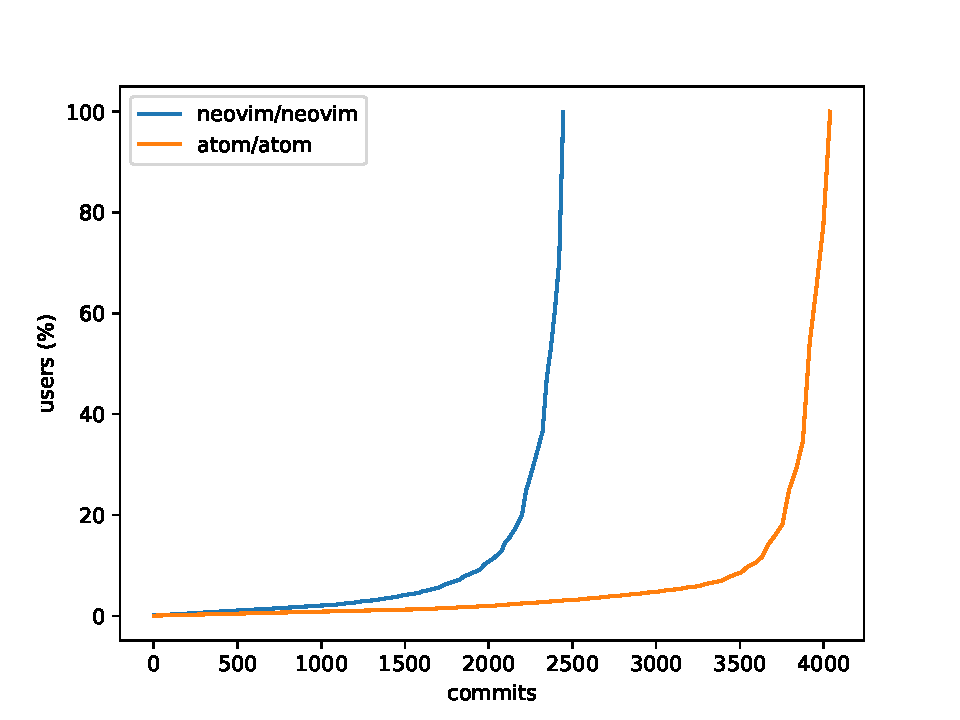
\includegraphics[width=1\textwidth]{commits_dist}
		\caption{\dots each other.}
		\label{fig:commits_dist}
	\end{subfigure}%
	\begin{subfigure}{.5\textwidth}
		\centering
		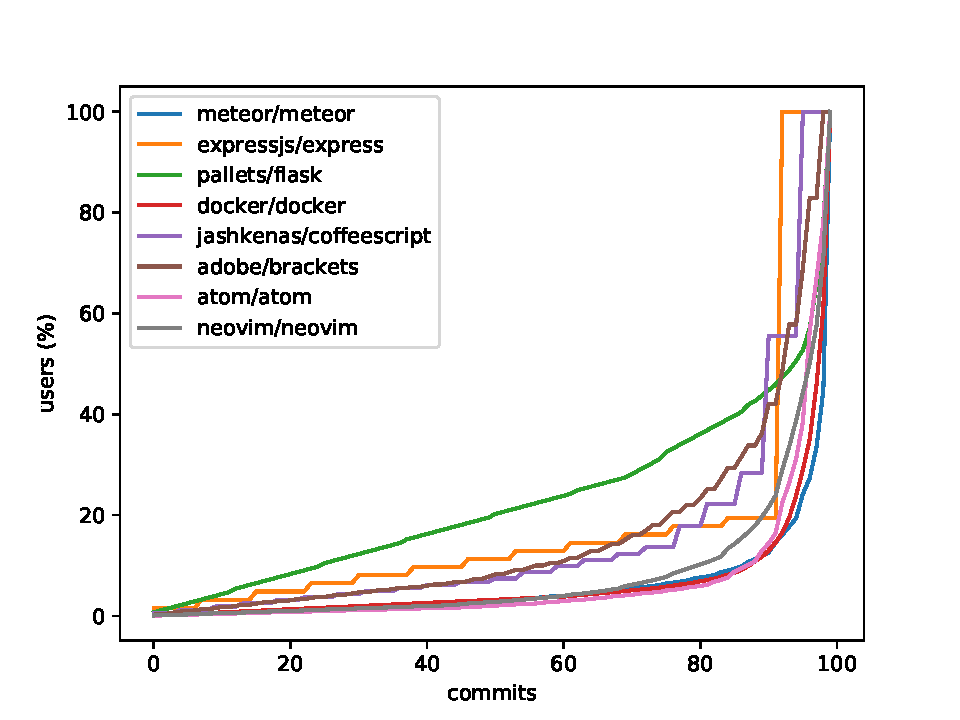
\includegraphics[width=1\textwidth]{all_commits_dist}
		\caption{\dots other popular OSS-projects.}
		\label{fig:all_commits_dist}
	\end{subfigure}
\end{figure}

\begin{figure}[!h]
	\centering
	\caption{Additions distribution compared to\dots}
	\begin{subfigure}{.5\textwidth}
		\centering
		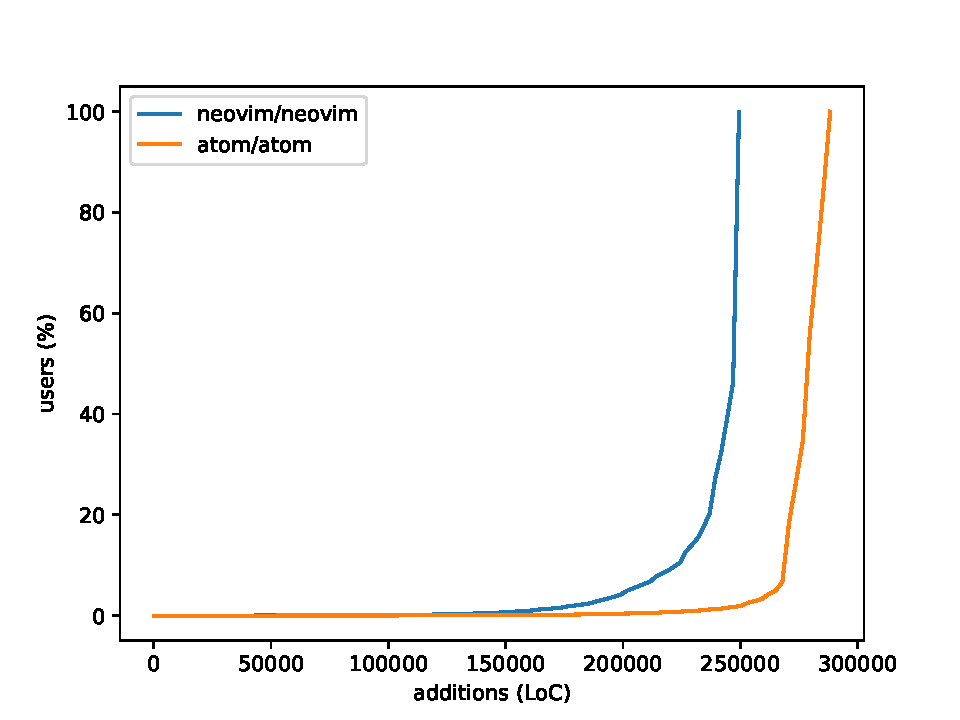
\includegraphics[width=1\textwidth]{additions_dist}
		\caption{\dots each other.}
		\label{fig:additions_dist}
	\end{subfigure}%
	\begin{subfigure}{.5\textwidth}
		\centering
		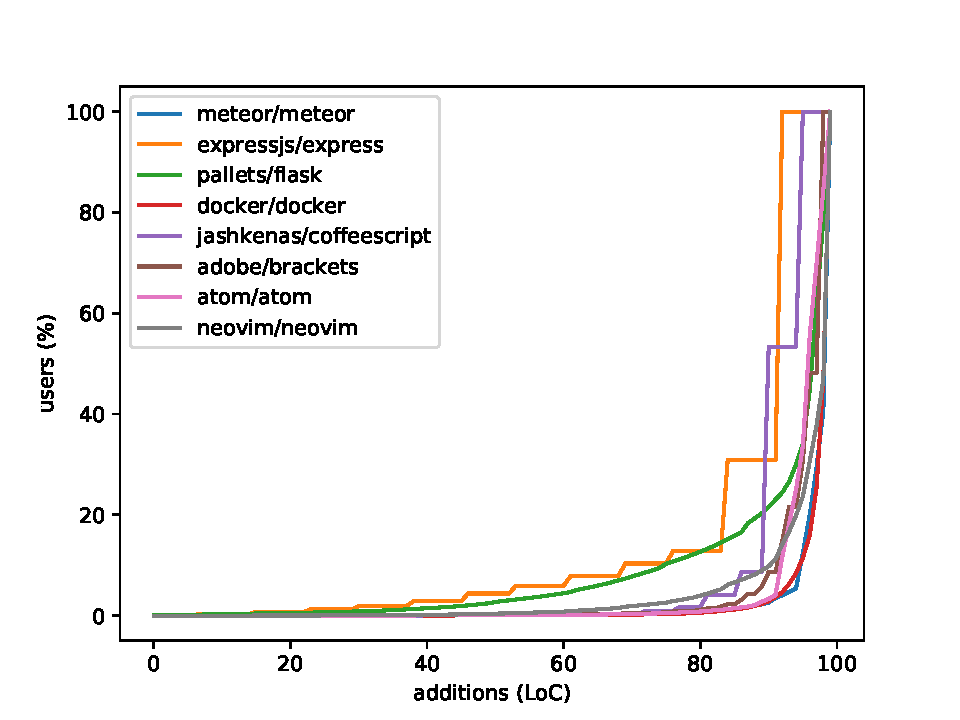
\includegraphics[width=1\textwidth]{all_additions_dist}
		\caption{\dots other popular OSS-projects.}
		\label{fig:all_additions_dist}
	\end{subfigure}
\end{figure}

\begin{figure}[!h]
	\centering
	\caption{Deletions distribution compared to\dots}
	\begin{subfigure}{.5\textwidth}
		\centering
		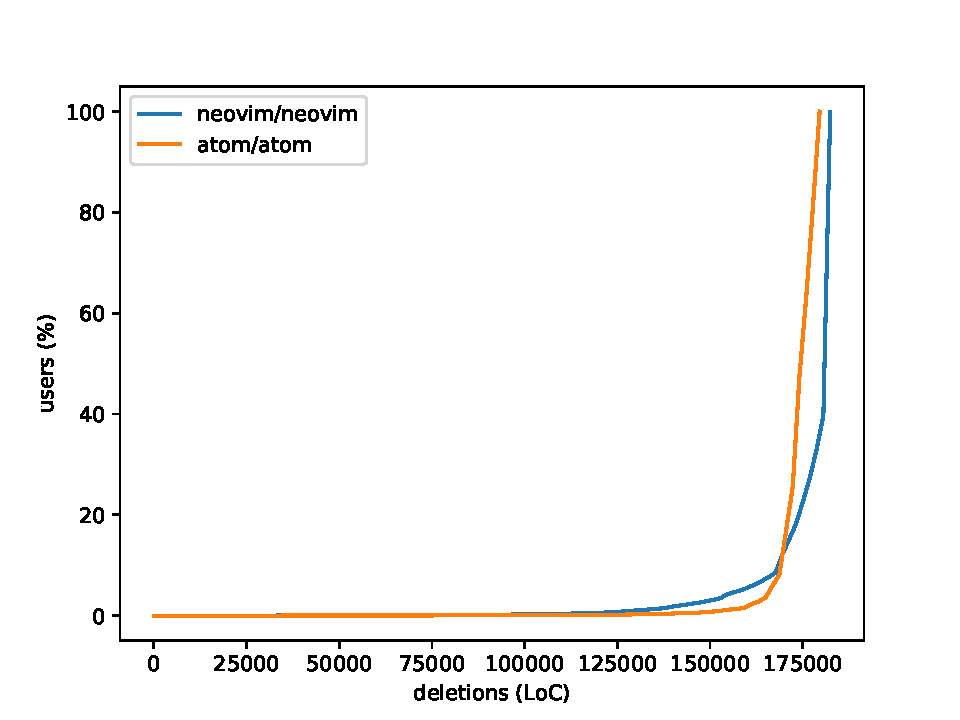
\includegraphics[width=1\textwidth]{deletions_dist}
		\caption{\dots each other.}
		\label{fig:deletions_dist}
	\end{subfigure}%
	\begin{subfigure}{.5\textwidth}
		\centering
		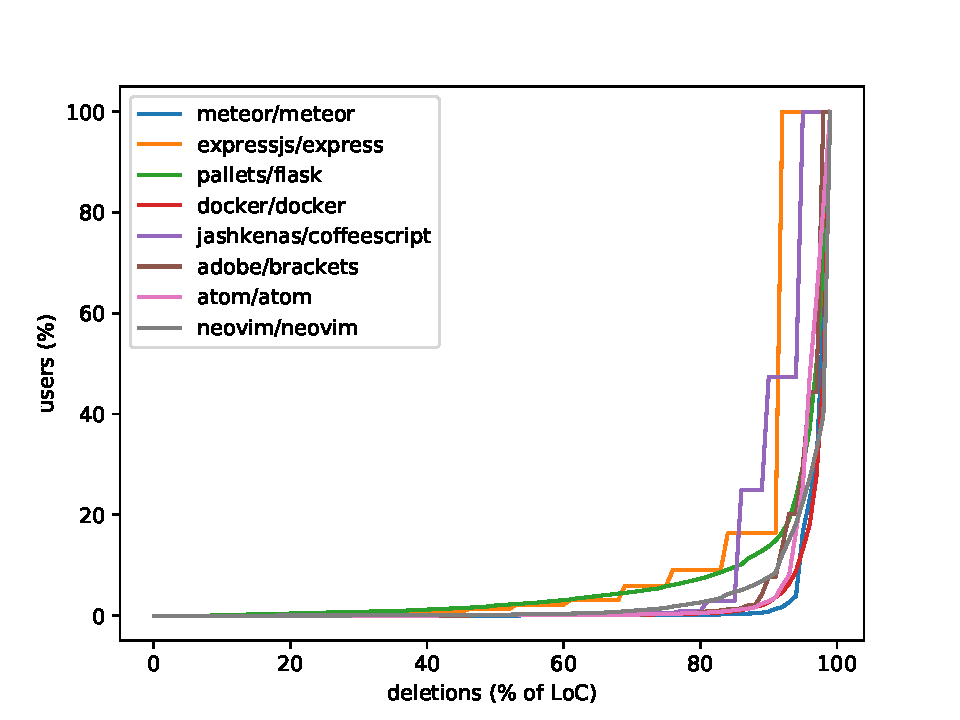
\includegraphics[width=1\textwidth]{all_deletions_dist}
		\caption{\dots other popular OSS-projects.}
		\label{fig:all_deletions_dist}
	\end{subfigure}
\end{figure}

\FloatBarrier
\subsubsection{Feature Proposers \& Problem Reporters (D2 \& D3)}
The amount of feature proposers were 108 for the two projects as seen in Table~\ref{tab:other_contributors}. The amount of problem reporters were 50 for the two projects as seen in Table~\ref{tab:other_contributors}. A majority, around 60\%, of the feature proposers and problem reporters did more than one proposal or report and the remaining 40\% did only one report each as seen in Figures~\ref{fig:feature_proposers} and~\ref{fig:problem_reporters}. Compared to other popular OSS-projects Atom and Neovim can be considered similar as seen in Tables~\ref{fig:all_feature_proposers} and~\ref{fig:all_problem_reporters}.
\begin{table}[h]
	\centering
	\begin{tabular}{ | l | c | c |}
		\hline
		\textbf{Data Type} 			& \textbf{Atom} 	& \textbf{Neovim}	\\\hline
		Amount of feature proposers	& 108		& 50		 		\\\hline
		Amount of problem reporters	& 230		& 141		 	\\
		\hline
	\end{tabular}
	\caption{Showing amount of feature proposers.}
	\label{tab:other_contributors}
\end{table}

\begin{figure}[!h]
	\centering
	\caption{Distribution of feature proposals over users compared to\dots}
	\begin{subfigure}{.5\textwidth}
		\centering
		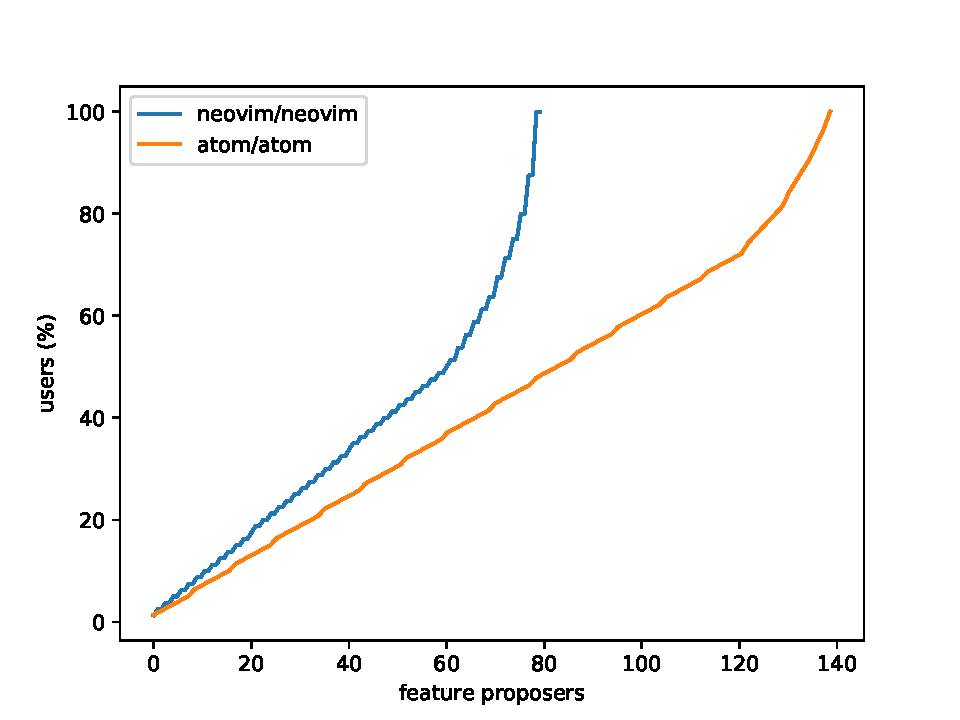
\includegraphics[width=1\textwidth]{feature_proposers_dist}
		\caption{\dots each other.}
		\label{fig:feature_proposers}
	\end{subfigure}%
	\begin{subfigure}{.5\textwidth}
		\centering
		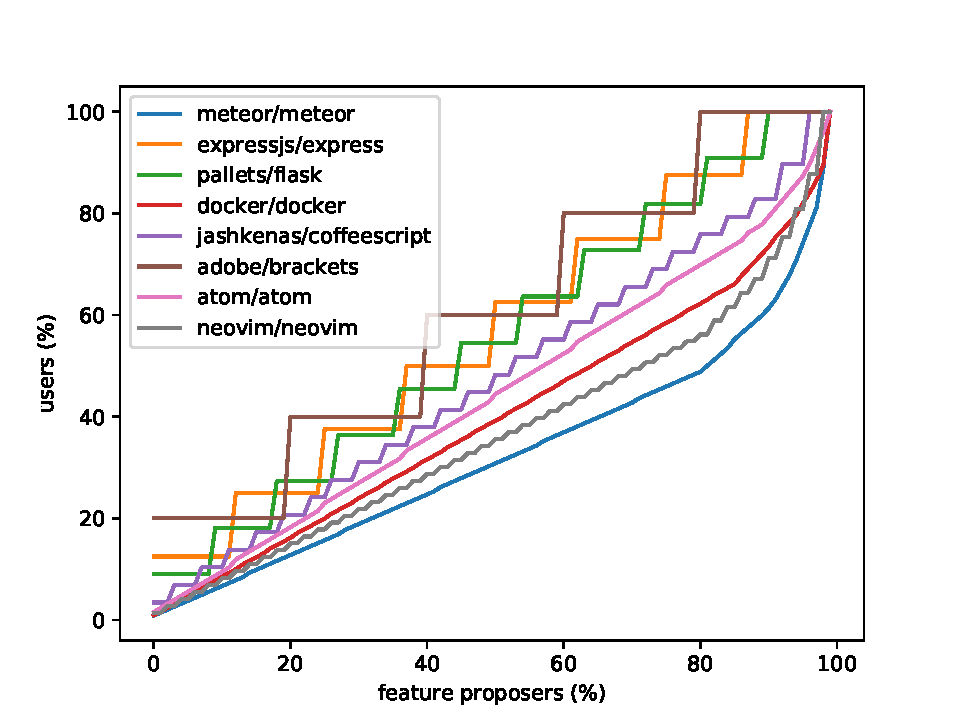
\includegraphics[width=1\textwidth]{all_feature_proposers_dist}
		\caption{\dots other popular OSS-projects.}
		\label{fig:all_feature_proposers}
	\end{subfigure}
\end{figure}

\begin{figure}[!h]
	\centering
	\caption{Distribution of problem reports over users compared to\dots}
	\begin{subfigure}{.5\textwidth}
		\centering
		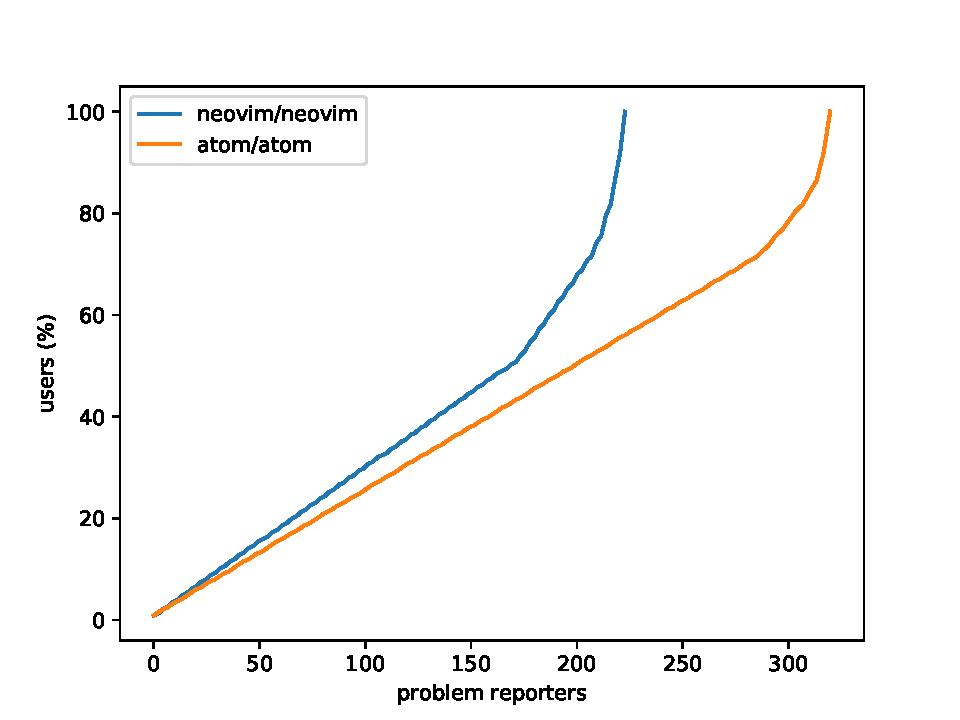
\includegraphics[width=1\textwidth]{problem_reporters_dist}
		\caption{\dots each other.}
		\label{fig:problem_reporters}
	\end{subfigure}%
	\begin{subfigure}{.5\textwidth}
		\centering
		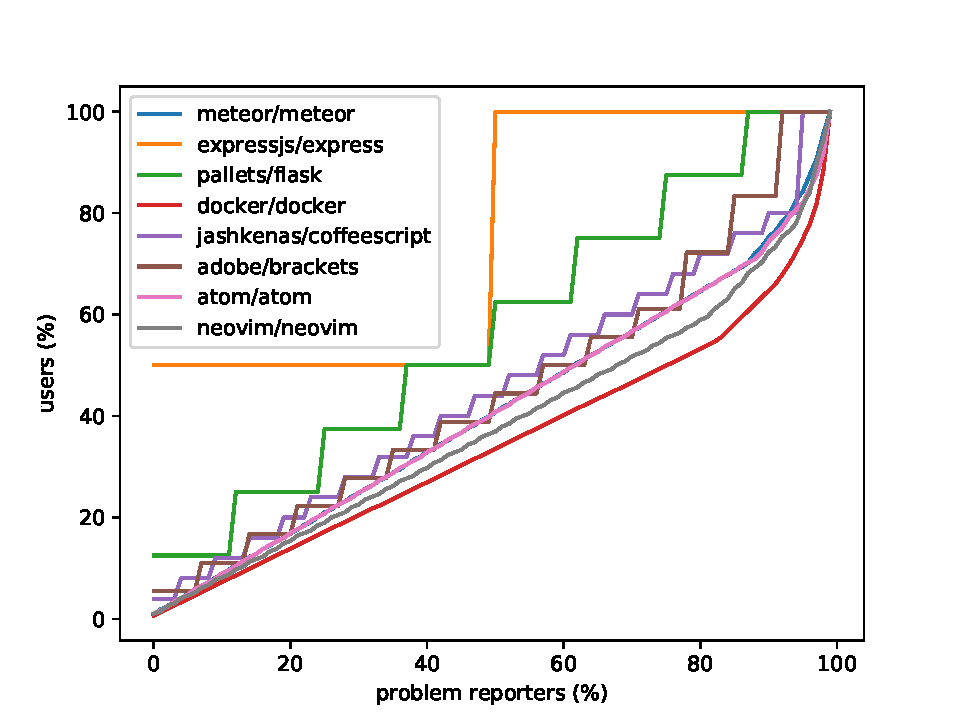
\includegraphics[width=1\textwidth]{all_problem_reporters_dist}
		\caption{\dots other popular OSS-projects.}
		\label{fig:all_problem_reporters}
	\end{subfigure}
\end{figure}

\FloatBarrier
\subsubsection{Defect Repair Time (D4)}
The two projects differed in the amount of defects repaired and the repair time, with Atom having almost twice as many defects, seen in Table~\ref{tab:defects} and a longer repair time, seen in Table~\ref{tab:repair_times}.
\begin{table}[h]
	\centering
	\begin{tabular}{ | l | c | c |}
		\hline
		\textbf{Data Type} 	& \textbf{Atom} 	& \textbf{Neovim}	\\\hline
		Amount defects		& 271		& 148		 	\\
		\hline
	\end{tabular}
	\caption{Showing amount of reported defects.}
	\label{tab:defects}
\end{table}

\begin{table}[h]
	\centering
	\begin{tabular}{ | l | c | c |}
		\hline
		\textbf{Data Type} 	& \textbf{Atom} 	& \textbf{Neovim}	\\\hline
		Average 			& 200 		& 151 			\\\hline
		Median	 		& 81			& 82 				\\\hline
		Highest			& 1098		& 807			\\\hline
		Lowest			& <1			& <1		 		\\
		\hline
	\end{tabular}
	\caption{Showing repair time measured in days.}
	\label{tab:repair_times}
\end{table}

\FloatBarrier
\subsection{Detailed Data}
\label{sec:detaileddata}
In previous section Overview Data~\ref{stat_data} we described overview data to show you that the the projects are on the same level for this comparison to be more accurate. We also showed you the two projects in a bigger picture with a comparison towards several other general known open source projects that can be found on Github.

In this section we will present to you the detailed data that we have collected from the Atom project and the Neovim project. The different data categories that we have investigated are described in section~\ref{subsec:data}. The raw collected data can be found in Appendix~\ref{ap:raw_detailed_data}.

\subsubsection{Feature Proposals (D5)}
The results of feature proposals displayed in Tables~\ref{tab:proposals_atom} and~\ref{tab:proposals_neovim} shows the amount of proposals made by individual users categorised as core developers, peripheral developers and end users. From this data we can summarise that there were a total of 20 feature proposals in the Atom project and 26 proposals in the Neovim project. Proposals from core developers in the Atom project adds up to a total of 4 and in the Neovim project they are a total of 12. Proposals made from contribution developers where in the Atom project a total of 12 in contrast to the Neovim project which had 11. Regarding proposals from end users the Atom project had 4 and the Neovim project had a total of 3.

In Table~\ref{tab:proposals_group} we can also see the number of unique users that that proposed a feature in each category in each project.The total amount of unique users among core developers ( core dev ) where 2 in the Atom project and 7 in the Neovim project. The biggest spread of unique users proposing features in both project are from the category peripheral developers (dev) where Atom had a total of 9 unique peripheral developers and Neovim had a total of 10. In the category of end users all feature proposals could be mapped to unique users came from proposals from end users did not where only unique events where Atom had 4 end users proposing features and Neovim had a total of 3.

\begin{table}[h]
	\centering
	\begin{tabular}{ | l | c | c |}
		\hline
		\textbf{Username} 	& \textbf{Feature Proposals}	& \textbf{User Status}	\\\hline
		damieng	 		& 3		 				& core developer		\\\hline
		celrenheit	 		& 2		 				& peripheral developer	\\\hline
		codingbelief	 	& 2		 				& peripheral developer	\\\hline
		fracalo	 		& 2		 				& peripheral developer	\\\hline
		mnquintana	 	& 1		 				& core developer 		\\\hline
		bgriffith	 		& 1		 				& peripheral developer	\\\hline
		caleb531	 		& 1		 				& peripheral developer	\\\hline
		astrojie	 		& 1		 				& peripheral developer	\\\hline
		alhadis	 		& 1		 				& peripheral developer	\\\hline
		kevindeleon	 	& 1		 				& peripheral developer	\\\hline
		MichaelAquiliana	& 1		 				& peripheral developer	\\\hline
		boustanihani	 	& 1		 				& end user 			\\\hline
		jamesonquinn	 	& 1		 				& end user 			\\\hline
		jesseleite	 		& 1		 				& end user			\\\hline
		karai17	 		& 1		 				& end user			\\
		\hline
	\end{tabular}
	\caption{Showing Atom users with amount of feature proposals.}
	\label{tab:proposals_atom}
\end{table}

\begin{table}[h]
	\centering
	\begin{tabular}{ | l | c | c |}
		\hline
		\textbf{Username} 	& \textbf{Feature Proposals}	& \textbf{User Status}	\\\hline
		bfredl			& 4 						& core developer 		\\\hline
		justinmk			& 2 						& core developer 		\\\hline
		tweekmonster 		& 2 						& core developer 		\\\hline
		shougo 			& 2 						& peripheral developer	\\\hline
		Splinterofchaos 	& 1						& core developer 		\\\hline
		jamessan 			& 1 						& core developer 		\\\hline
		elmart 			& 1 						& core developer 		\\\hline
		tarruda 			& 1 						& core developer 		\\\hline
		mtortonesi 		& 1 						& peripheral developer	\\\hline
		shazow 			& 1 						& peripheral developer	\\\hline
		rygwdn 			& 1 						& peripheral developer	\\\hline
		tony 				& 1 						& peripheral developer	\\\hline
		cyphar 			& 1 						& peripheral developer	\\\hline
		joshtriplett 		& 1 						& peripheral developer	\\\hline
		nhooyr 			& 1 						& peripheral developer	\\\hline
		ZyX-I 			& 1 						& peripheral developer	\\\hline
		equalsraf			& 1		 				& peripheral developer	\\\hline
		sunaku 			& 1 						& end user 			\\\hline
		abstiles			& 1		 				& end user 			\\\hline
		mmlb 			& 1 						& end user 			\\
		\hline
	\end{tabular}
	\caption{Showing Neovim users with amount of feature proposals.}
	\label{tab:proposals_neovim}
\end{table}
\begin{table}[h]
	\centering
	\begin{tabular}{ | l | c | c |}
		\hline
		\textbf{User Group} 	& \textbf{Atom} 	& \textbf{Neovim}	\\\hline
		core devs 			& 2 			& 7 				\\\hline
		devs	 			& 9			& 10 				\\\hline
		end-users			& 4			& 3				\\
		\hline
	\end{tabular}
	\caption{Showing amount of feature proposers in user groups.}
	\label{tab:proposals_group}
\end{table}

\FloatBarrier
\subsubsection{Feature Origin Categories (D6)}
Presented in this section are the result for proposals in category A, B and C described in section~\ref{subsec:data}.
\begin{table}[h]
	\centering
	\begin{tabular}{ | l | c | c | c | c |}
		\hline
		\textbf{Proposal Category} 	& \textbf{Atom} 	& \textbf{Neovim}	\\\hline
		A						& 16 			& 18				\\\hline
		B		 				& 2			& 6 	 			\\\hline
		C						& 4			& 3				\\\hline
		tot. 						& 22 			& 27 				\\
		\hline
	\end{tabular}
	\caption{Showing amount of proposals for each category.}
\end{table}

\FloatBarrier
\subsubsection{Feature Acknowledgement (D7)}
The two tables~\ref{tab:acknowledgements_atom} and~\ref{tab:acknowledgements_neovim} below presents detailed data for feature acknowledgement~\ref{subsec:data}. The tables includes data regarding unique user status (peripheral developer or core developer), the amount of features they have acknowledge during the time period and the unique username. Table~\ref{tab:acknowledgements_atom} presents detailed data from the Atom project and Table~\ref{tab:acknowledgements_neovim} present detailed data from the Neovim project.

\begin{table}[h]
	\centering
	\begin{tabular}{ | l | c | c |}
		\hline
		\textbf{Username} 	& \textbf{Feature Acknowledgements}	& \textbf{User Status}	\\\hline
		fracalo 			& 4 								& peripheral developer	\\\hline
		bastillian 			& 3 								& peripheral developer	\\\hline
		kuychaco 			& 2 								& core developer 		\\\hline
		damieng 			& 2 								& core developer 		\\\hline
		50Wliu 			& 2 								& core developer 		\\\hline
		svanharmelen 		& 2 								& peripheral developer	\\\hline
		as-cii 			& 1 								& core developer 		\\\hline
		lee-dohm 			& 1 								& core developer 		\\\hline
		simurai 			& 1 								& core developer 		\\\hline
		izuzak 			& 1 								& core developer 		\\\hline
		codingbelief 		& 1 								& peripheral developer	\\\hline
		benogle 			& 1 								& peripheral developer	\\\hline
		nathansobo 		& 1 								& peripheral developer	\\
		\hline
	\end{tabular}
	\caption{Showing Atom users with amount of feature acknowledgements.}
	\label{tab:acknowledgements_atom}
\end{table}
\begin{table}[h]
	\centering
	\begin{tabular}{ | l | c | c |}
		\hline
		\textbf{Username} 	& \textbf{Feature Acknowledgements}	& \textbf{User Status}	\\\hline
		justinmk 			& 12 								& core developer 		\\\hline
		bfredl 			& 4	 							& core developer 		\\\hline
		tarruda 			& 2 								& core developer 		\\\hline
		jamessan 			& 2 								& core developer 		\\\hline
		tweekmonster 		& 2 								& core developer 		\\\hline
		alexgenco 		& 2 								& peripheral developer	\\\hline
		mhinz 			& 1 								& core developer 		\\\hline
		tjdevries			& 1 								& peripheral developer	\\\hline
		shougo 			& 1 								& peripheral developer	\\
		\hline
	\end{tabular}
	\caption{Showing Neovim users with amount of feature acknowledgements.}
	\label{tab:acknowledgements_neovim}
\end{table}

\FloatBarrier
\subsubsection{First Implementation of Feature (D8)}
This section presents the collected detailed data for whom a first feature implementation came from. Table~\ref{tab:implementation_atom} presents this data for the Atom project and Table~\ref{tab:implementation_neovim} presents the data for the Neovim project. Both Table~\ref{tab:implementation_atom} and Table~\ref{tab:implementation_neovim} includes data regarding the amount of first implementation from a unique user, the status of that unique user (core developer or peripheral developer) and the unique username.
\begin{table}[h]
	\centering
	\begin{tabular}{ | l | c | c |}
		\hline
		\textbf{Username} 	& \textbf{First Feature Implementations}	& \textbf{User Status}	\\\hline
		damieng 			& 3 								& core developer 		\\\hline
		bastillian 			& 3 								& peripheral developer	\\\hline		
		50Wliu			& 1 								& core developer 		\\\hline
		kuychaco 			& 1 								& core developer 		\\\hline
		wil93 			& 1 								& core developer 		\\\hline
		alhadis 			& 1 								& peripheral developer	\\\hline
		astrojie 			& 1 								& peripheral developer	\\\hline
		caleb531 			& 1 								& peripheral developer	\\\hline
		codingbelief 		& 1 								& peripheral developer	\\\hline
		danjordan 		& 1 								& peripheral developer	\\\hline
		esdoppio 			& 1 								& peripheral developer	\\\hline
		fracalo 			& 1 								& peripheral developer	\\\hline
		jtokoph 			& 1 								& peripheral developer	\\\hline
		kevindeleon 		& 1 								& peripheral developer	\\\hline
		MichaelAquilina 	& 1 								& peripheral developer	\\\hline
		timkelty 			& 1 								& peripheral developer	\\
		\hline
	\end{tabular}
	\caption{Showing Atom users with amount of first feature implementations.}
	\label{tab:implementation_atom}
\end{table}
\begin{table}[h]
	\centering
	\begin{tabular}{ | l | c | c |}
		\hline
		\textbf{Username} 	& \textbf{First Feature Implementations}	& \textbf{User Status}	\\\hline
		justinmk			& 10 								& core developer 		\\\hline
		bfredl			& 8 								& core developer 		\\\hline
		tweekmonster		& 2 								& core developer 		\\\hline
		jamessan			& 2 								& core developer 		\\\hline
		alexgenco			& 1		 						& peripheral developer	\\\hline
		nhooyr			& 1 								& peripheral developer	\\\hline
		shougo			& 1 								& peripheral developer	\\\hline
		ZyX-I			& 1		 						& peripheral developer	\\
		\hline
	\end{tabular}
	\caption{Showing Neovim users with amount of first feature implementations.}
	\label{tab:implementation_neovim}
\end{table}
\FloatBarrier
\newpage
\section{Analysis}
\label{sec:analysis}
In the previous section, we presented and described the results from our overview and detailed data gathering that we have conducted.
In this section we will analyse our results presented in the previous section. The analysis consist of three parts: validate the selection of cases and identify similarities and differences in requirement elicitation process.

\subsection{Validity of Selected Cases}
From the results we can identify two things. First, the two projects are similar in size on a number of aspects, as seen in Table~\ref{tab:contributors_amount} and Figures~\ref{fig:additions_dist},~\ref{fig:deletions_dist},~\ref{fig:feature_proposers} and~\ref{fig:problem_reporters}. Second, the distribution of the gathered overview data are very similar both between the projects, but also compared to other popular OSS-projects as seen in Figures~\ref{fig:all_commits_dist},~\ref{fig:all_additions_dist},~\ref{fig:all_deletions_dist},~\ref{fig:all_feature_proposers} and~\ref{fig:all_problem_reporters}. With this information the two selected projects can be considered suitable for comparison on requirement elicitation.

The difference in amounts of commits as seen in Figure~\ref{fig:commits_dist} could, as mentioned before in section~\ref{sec:case_selection}, be a difference in how the two projects use commits.

\subsection{Identify Similarities and Differences from Detailed Data}

In general, participants in a open source software development show a strong sense of engagement in, and ownership of, the project, without having any particular reward for the time they spent on contributing to the development. In the case of Atom and Neovim there are no exceptions however within this engagement among participants we have seen certain differences and similarities within feature proposals, origin, acknowledgement and in the first implementation of a feature the engagement among participants.

% Feature Proposals
The results from feature proposals shows us the amount of proposals made by individual users categorised in core developers, peripheral developers and end users. From this data we can summarize that there where a total of 20 feature proposals in the Atom project and 26 proposals in the Neovim project. Proposals from core developers in the Atom project adds up to a total of 4 and in the Neovim project they are a total of 12. Proposals made from peripheral developers where a total of 12 in the Atom project in contrast to the Neovim project which had a total of 11. Regarding proposals from end users the Atom project had 4 and the Neovim project had a total of 3.

\begin{table}[h]
	\centering
	\begin{tabular}{ | c | }
		\hline
		\\
		In Neovim around 50\% of the feature proposals was from core developers. \\In Atom they were only 20\%.\\
		\\
		\hline
	\end{tabular}
	\label{tab:more_devs_in_neovim_analysis}
\end{table}

We can also see the number of unique users that proposed a feature in each category for each project.The total amount of unique users among core developers where 2 in the Atom project and 7 in the Neovim project. The biggest spread of unique users proposing features in both project are from the category peripheral developers where Atom had a total of 9 and Neovim had a total of 10. In the category of end users all feature proposals could be mapped to unique users.

\begin{table}[h]
	\centering
	\begin{tabular}{ | c | }
		\hline
		\\
		The amount of suggestions per user is approximately the same for the two projects.\\
		\\
		\hline
	\end{tabular}
	\label{tab:same_suggestions_analysis}
\end{table}

% Feature Origin
Looking into the detailed data for feature origin it was in both cases clear that the majority of proposals originated from a developer's personal experience or his knowledge of user needs, 72,7\% in the Atom Project and 66,7\% in the Neovim Project. There where 9.1\% proposals coming from end users in the Atom project and 2,2\% in the Neovim project. In the aspect of features that derives from competing products there where a also a minor difference, where Atom had 1,8\% and Neovim had 1,1\% of the feature proposals.

\begin{table}[h]
	\centering
	\begin{tabular}{ | c | }
		\hline
		\\
		Feature origin categories was for both projects approximately the same.\\
		\\
		\hline
	\end{tabular}
	\label{tab:same_suggestions_analysis}
\end{table}

% Feature Acknowledgement
Acknowledgment of features are the single most interesting aspect of the detailed data. In our results we can see that core developers in the Atom project stands for 45,5\% of the acknowledgments compared to the 85,2\% in the Neovim project. This means that 55,5\% of the feature acknowledgements came from peripheral developers in the Atom project and 14,5\% in the Neovim. There are two aspects that makes these numbers interesting. First several peripheral developers in both projects have the authorities to acknowledge a feature for implementation, for what we can see, without a core developers involvement. The Second interesting finding is the fact that the Atom project allow more than half of their features to be acknowledge by peripheral developers while the Neovim project only have 14,5\% acknowledgments by peripheral developers. Furthermore the developers in the Atom project that made the most acknowledgements were peripheral developers while the Neovim project had core developers in the top.
\begin{table}[h]
	\centering
	\begin{tabular}{ | c | }
		\hline
		\\
		Peripheral developers are in both projects allowed to acknowledge feature proposals.
		\\ \\
		In Atom 55,5\% of the feature acknowledgements came from peripheral developers.\\ In Neovim the number was only 14,5\%.\\
		\\
		
		\hline
	\end{tabular}
	\label{tab:acknowledgements_analysis}
\end{table}

We also found that there are a significant spread among acknowledgement from unique developers in the projects, in the Neovim the core developer ''justinmk'' stands for 44,4\% of the feature acknowledgements while the developer ''fracalo'' in the Atom project stands for 18,2\%.

% First Implementation of feature
Moving on to analyse the first implementation of a feature we can confirm that from the features that had been proposed in the Atom project 27,3\% of them where first implemented by a core developer and 72,7\% where implemented by a peripheral developer. The Neovim project on the other hand had 86,6\% of first feature implementation done by core developers and 15,4\% from peripheral developers. Furthermore the data also shows that that the core developer ''justinmk'' stands for 38,5\% of the first feature implementations in the Neovim project and the top spot with 13,6\% in Atom is shared between the core developer ''damieng'' and the peripheral developer ''bastillian''. Overall there are a total of 12 peripheral developers and 4 core developers in the Atom project doing first implementation of a feature while Neovim has a total of 4 core developers and 4 peripheral developers.
\begin{table}[h]
	\centering
	\begin{tabular}{ | c | }
		\hline
		\\
		In Atom the majority of feature implementations were done by peripheral developers.\\ For Neovim it was the opposite.\\
		\\
		\hline
	\end{tabular}
	\label{tab:feature_implementations_analysis}
\end{table}

%\subsection{Other Findings}
	%implementation took under a day to implement no time when the proposal
 	%Time to implementation in the aspects of the proposer

\newpage
\section{Discussion}
\label{section:discussion}
%Section intro
In section \ref{sec:intro} we have present the problem, purpose, contribution and approach for this thesis. Furthermore in section \ref{subsec:background} we introduce the research area and describe the related work within the area. Based on these facts and thoughts a total of three research question where framed and presented in section \ref{sec:rq}. 

In this section we will discuss our findings in the previous section, their implications and their relevance to our first two research questions. Then we will discuss, based on the first two research questions, the answer for our third research question. We consider the answers to the first two questions to be conclusive, and the answer for our third research question to be speculative.

\subsection{Conclusive}
\label{subsection:discussion_conclusive}
%Answer Research question 1
The research questions \emph{What are the characteristics of community-driven OSS development?} and \emph{What are the characteristics of firm-driven OSS development?} will be discussed in this section. A summary of the differences between the both cases will be presented and further more a conclusion will be framed for each research question based on the result data in section~\ref{sec:detaileddata}.

From our analysis we can see that the firm driven project, Atom, has, when compared to the community-driven project Neovim, the following differences: (1) in Atom, core developers did only 20\% of the feature proposals, in Neovim it was around 50\%; (2) in Atom, 55,5\% of feature acknowledgements came from peripheral developers, in Neovim it was 14,5\%; (3) in Atom, 72,7\% of first implementations was done by peripheral developers, in Neovim it was 15,4\%.

% answer RQ1 & RQ2
The differences mentioned in the paragraph above would imply the following for our research questions:
\begin{enumerate}[label=RQ\arabic*]
	\item \emph{What are the characteristics of community-driven OSS development?}
	
	In community-driven OSS development, core developers in projects tend to have a \textbf{high} presence in suggesting-, acknowledging- and implementing features.
	\item \emph{What are the characteristics of firm-driven OSS development?}
	
	In firm-driven OSS development, core developers in projects tend to have a \textbf{low} presence in suggesting-, acknowledging- and implementing features.
\end{enumerate}

Communities and firms have approximately the same end-user involvement which means that when firms consider to choose OSS-development they can look at any OSS-project to see how end-users are involved.

%Compare other studies
When comparing the results from this thesis to the article~\cite{Noll} the results shows that the majority of features are asserted by developers, based on either their personal experience, or knowledge of users needs. Therefore we can conclude that our results are general for several areas within the area of OSS development. Furthermore we also compare the results from our statistical data from section~\ref{stat_data} with the results from~\cite{Mockus2002a}, where we can see a similar pattern based on the schema we framed for overview data in section~\ref{subsec:data}.

\subsection{Speculative}
\label{sub:speculative}
%Peripheral developers participation F>C
From the differences that the we concluded in Section~\ref{subsection:discussion_conclusive} for research questions one and two, one could speculate in what they implicate. Looking at peripheral developer participation in firm-driven projects we can see that it's higher. That implicates that communities could have a higher peripheral developer participation which could result in; (1) increasing product customer value by having more developers working on improving the product; (2) increasing the actual development speed by having a greater number of developers; and (3) enabling core developers to focus on managing project and its future goals by relieving them of development work.

Furthermore from a firms perspective the participation from peripheral developers is already high. This could mean that firms choosing to use an OSS development approach instead of a proprietary development approach could (1) increase their development speed without increased costs by having more developers and (2) increasing product customer value by having more developers working on improving the product.

From the analysis we found more points regarding core and peripheral developers that both community and firm driven project could benefit from. The finding that we did concerns the distribution of task within a process and the actual definition of developers. According to previous research,~\cite{Noll, Joblin}, there is a clear line between the two kinds of developers within a project and the task they are held responsible for. From our result we can se a different type of pattern that does not follow along the lines of what previous research have defined. We found that acknowledgment, a core developer task, in several occasions where approved by peripheral developers. This anamoly in task distribution could imply that there are roles in these projects that are in need of a new definition. In the perspective from the two types of projects this thesis aim to support one could argue that these findings are an opportunity to engage developers in the project even further by giving them more important reachable roles than just core and peripheral developers. This could by itself lead to (1) better engagement within the group of developers and (2) this could also lead to better reputation among developers outside of the project due to the fact of a more reachable goal and opportunity within the project.

\subsection{Unforeseen complications}
% discuss Barcelona, peripheral developer acknowledge, maybe they are not peripheral?
When analysing the result we found that the definition we used to categorise core and peripheral developers might not be accurate, as mention in previous section~\ref{sub:speculative}. We notice this due to the fact that there where a high amount of peripheral developers that made acknowledgments in both of the projects, a task that according to earlier research should be in the hands of a core developer. Furthermore we investigated this unforeseen complication and found a resent study written by~\cite{Krishnamurthy2016} that brings forward a more in depth description in how developers should be defined and categorised.

%The result also showed that there were difference in the delegation of work in the projects, the core developers that we could define did not contribute as much code as the core developers in the Neovim project. However the Atom project had a more wider spread of the work between core developers and peripheral developers that where throughout the project while the Neovim project had a clear pattern of individual core developers doing more work than others in the project. There could be many reasons to why the difference are so clear in this matter and we can only discuss this matter since we don?t have the data to back up and confirm a correct statement. So to discuss the matter this could be a result of Atom having a firm behind them with more structure towards the projects whereas Neovim are driven by a core group of individuals that are driven to dedicate there hours to the project.

\newpage
\section{Conclusion and Suggestions for Future Work}
In this section we will summarise the answer for all three research questions. And then make suggestions for future work.
%Include the RQ's and answer them.

%Suggest future work within the area.
	% Redo this study but with a more accurate definition of pheripheral developer.

\newpage
\addcontentsline{toc}{section}{References}
\bibliographystyle{plain}
\bibliography{library,custom}
\newpage
\appendix
\section{Detailed Data Schema for Statistical Data}
\label{ap:detailed_data}
In this appendix we will give a detailed description for how we define each of the data type presented in the thesis. Before presenting the definitions we will explain some Git-terms.

\subsection*{Git-terms}
Git is, as mentioned in the thesis, a version control system. Below we present the Git-terms used to present the data schema definitions.

\begin{itemize}
	\item\texttt{commit}

	A set of changes to the source code. The \texttt{commit} always has an author and an ID, typically a message describing the \texttt{commit} is also included.
	\item\texttt{issue}

	An \texttt{issue} is a suggestion for improvement, task or question related to the project. An \texttt{issue} can be created by anyone. An \texttt{issue} can have the status \texttt{open} or \texttt{closed}.

	\item\texttt{label}

	An \texttt{issue} can optionally also have one or many \texttt{label}s. A \texttt{label} provides meta data to the \texttt{issue}. Projects can define their own labels, popular \texttt{label}s are for example \texttt{duplicate}, \texttt{enhancement} and \texttt{bug}.
\end{itemize}

\subsection*{Code contributor}
Any author of a \texttt{commit} to the project is a code contributor.
\subsection*{Feature proposal}
Any author of an \texttt{issue} to the project with the following criterias: (1) the \texttt{issue} is \texttt{label}ed as an enhancement, (2) the \texttt{issue} is not labeled as a duplicate and (3) the \texttt{issue} is \texttt{closed}.
\begin{enumerate}
	\setcounter{enumi}{1}
	\item If there are two \texttt{issues} proposing the same thing. One of them is labeled as a duplicate. We only need to count the one that is not.
	\item To ensure that the \texttt{issue} is in fact not a duplicate it needs to already be \texttt{closed}. This means that a user has seen the issue, and if it is a duplicate the user would have labeled it as such.
\end{enumerate}
\subsection*{Problem reporters}
Any author of a problem report which we define as an \texttt{issue} to the project with the following criterias: (1) the \texttt{issue} is \texttt{label}ed as an bug, (2) the \texttt{issue} is not labeled as a duplicate and (3) the \texttt{issue} is \texttt{closed}.
\begin{enumerate}
	\setcounter{enumi}{1}
	\item If there are two \texttt{issues} reporting the same thing. One of them is labeled as a duplicate. We only need to count the one that is not.
	\item To ensure that the \texttt{issue} is in fact not a duplicate it needs to already be \texttt{closed}. This means that a user has seen the issue, and if it is a duplicate the user would have labeled it as such.
\end{enumerate}
\subsection*{Defect repair time}
Defect repair time is the time between the creation of a problem report and when it was \texttt{closed}.

\newpage
\section{Libraries and Programmed Scripts}
\label{ap:scripts}
In this appendix we will present the libraries and main scripts used. To see the complete system please see our public Github repository found at: \url{https://github.com/FilipHarald/bachelor-thesis}.

\subsection*{Libraries}
\begin{itemize}
  \item\href{http://pygithub.readthedocs.io/}{\texttt{PyGithub}}


  This python library was used to communicate with Github through the Github API.
  \item\href{http://matplotlib.org/}{\texttt{Matplotlib}}

  This python library was used to visualize our results from the statistical data.
\end{itemize}

\subsection*{Main Scripts}
Below we present the two main scripts used to collect the data. The first, \texttt{code\_contributors.py}, collected data for D1. The second, \texttt{other\_contributors.py}, collected data for D2-D4.

\subsubsection*{\texttt{code\_contributors.py}}
\lstinputlisting[language=Python]{../data-collection-tools/code_contributors.py}
\subsubsection*{\texttt{other\_contributors.py}}
\lstinputlisting[language=Python]{../data-collection-tools/other_contributors.py}

\newpage
\section{Detail Results Raw Data}
\label{ap:raw_detailed_data}
In this appendix we present the raw data collected for D5-D7. The data can also be found at: \url{https://docs.google.com/spreadsheets/d/1HuNUuB8UeVbQUn4qeKSg7NY_QTHRG5_PlzuXJua196w/edit?usp=sharing}. First we present the data for Atom and then Neovim.
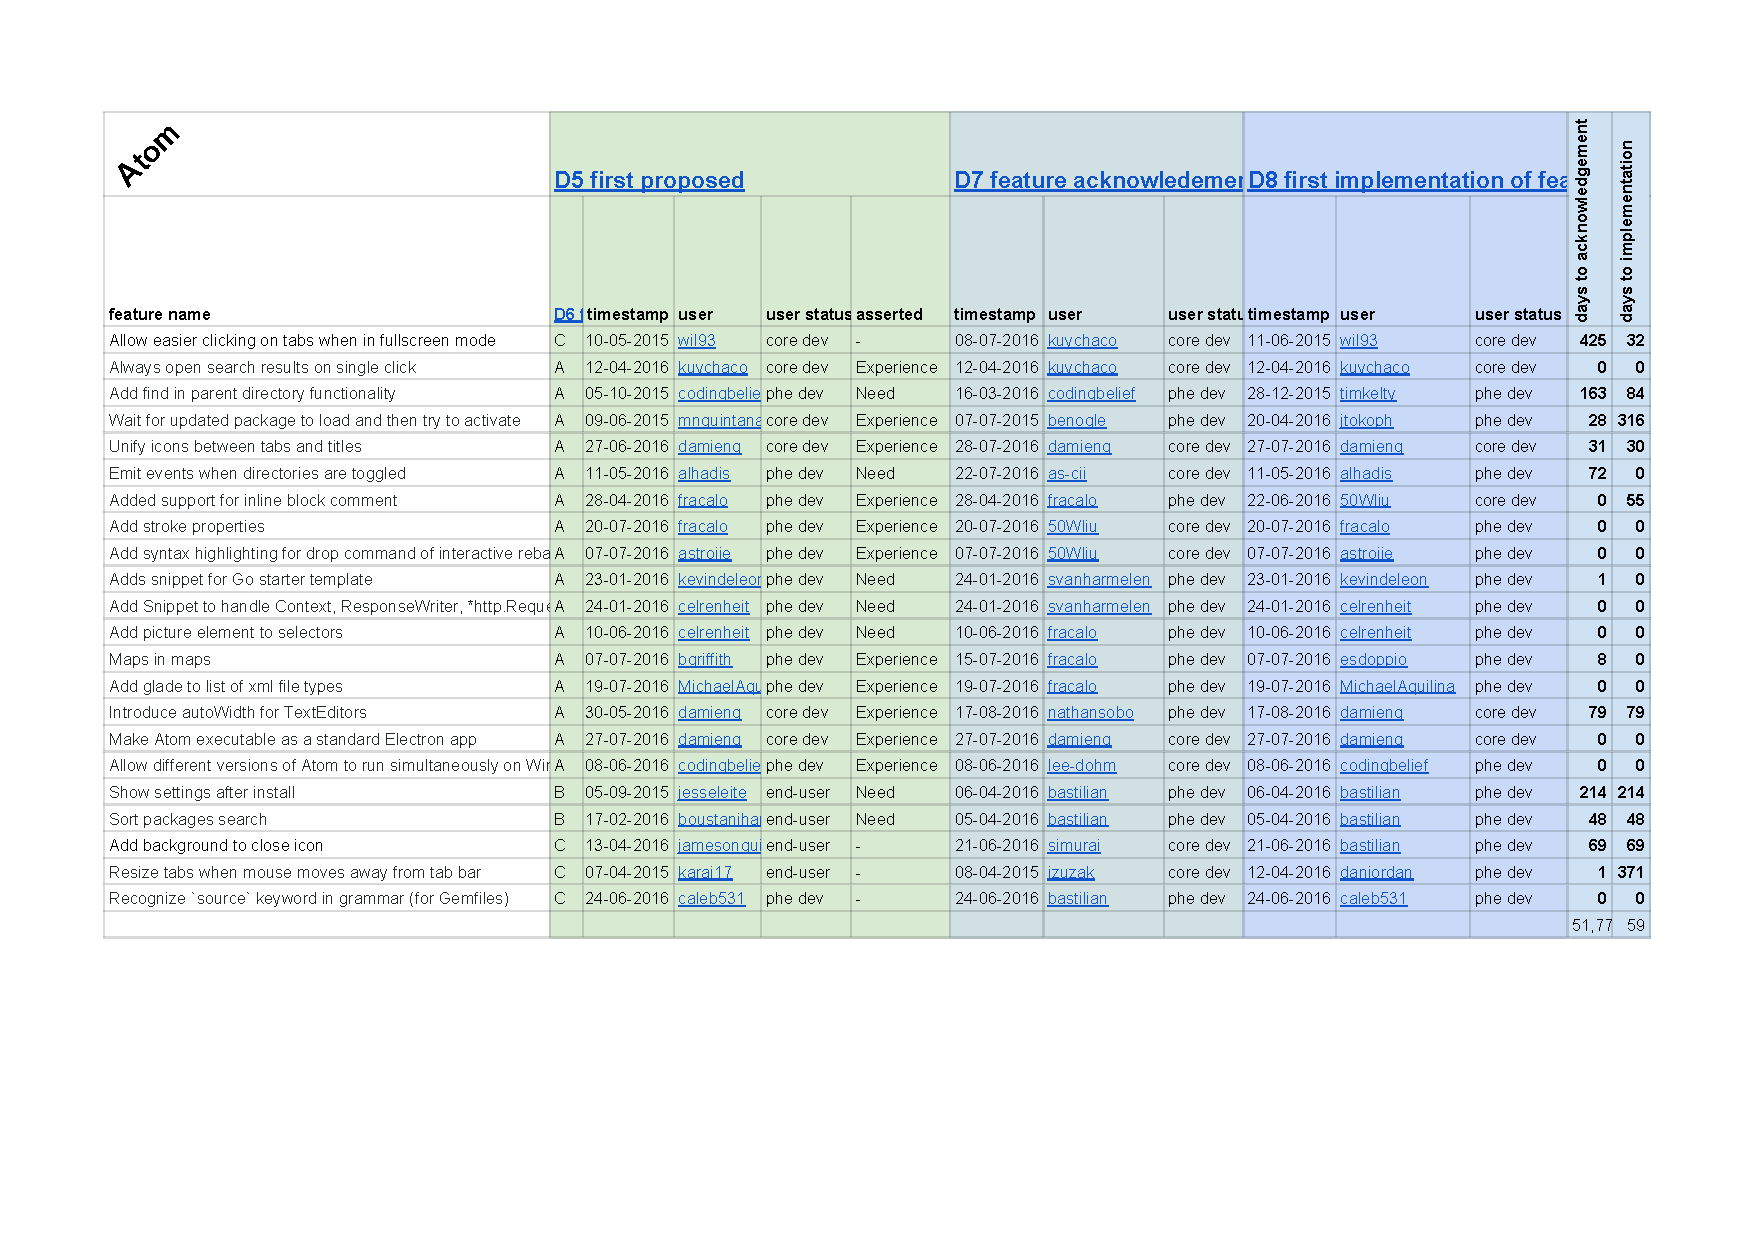
\includepdf{appendicies/detail_data_atom}
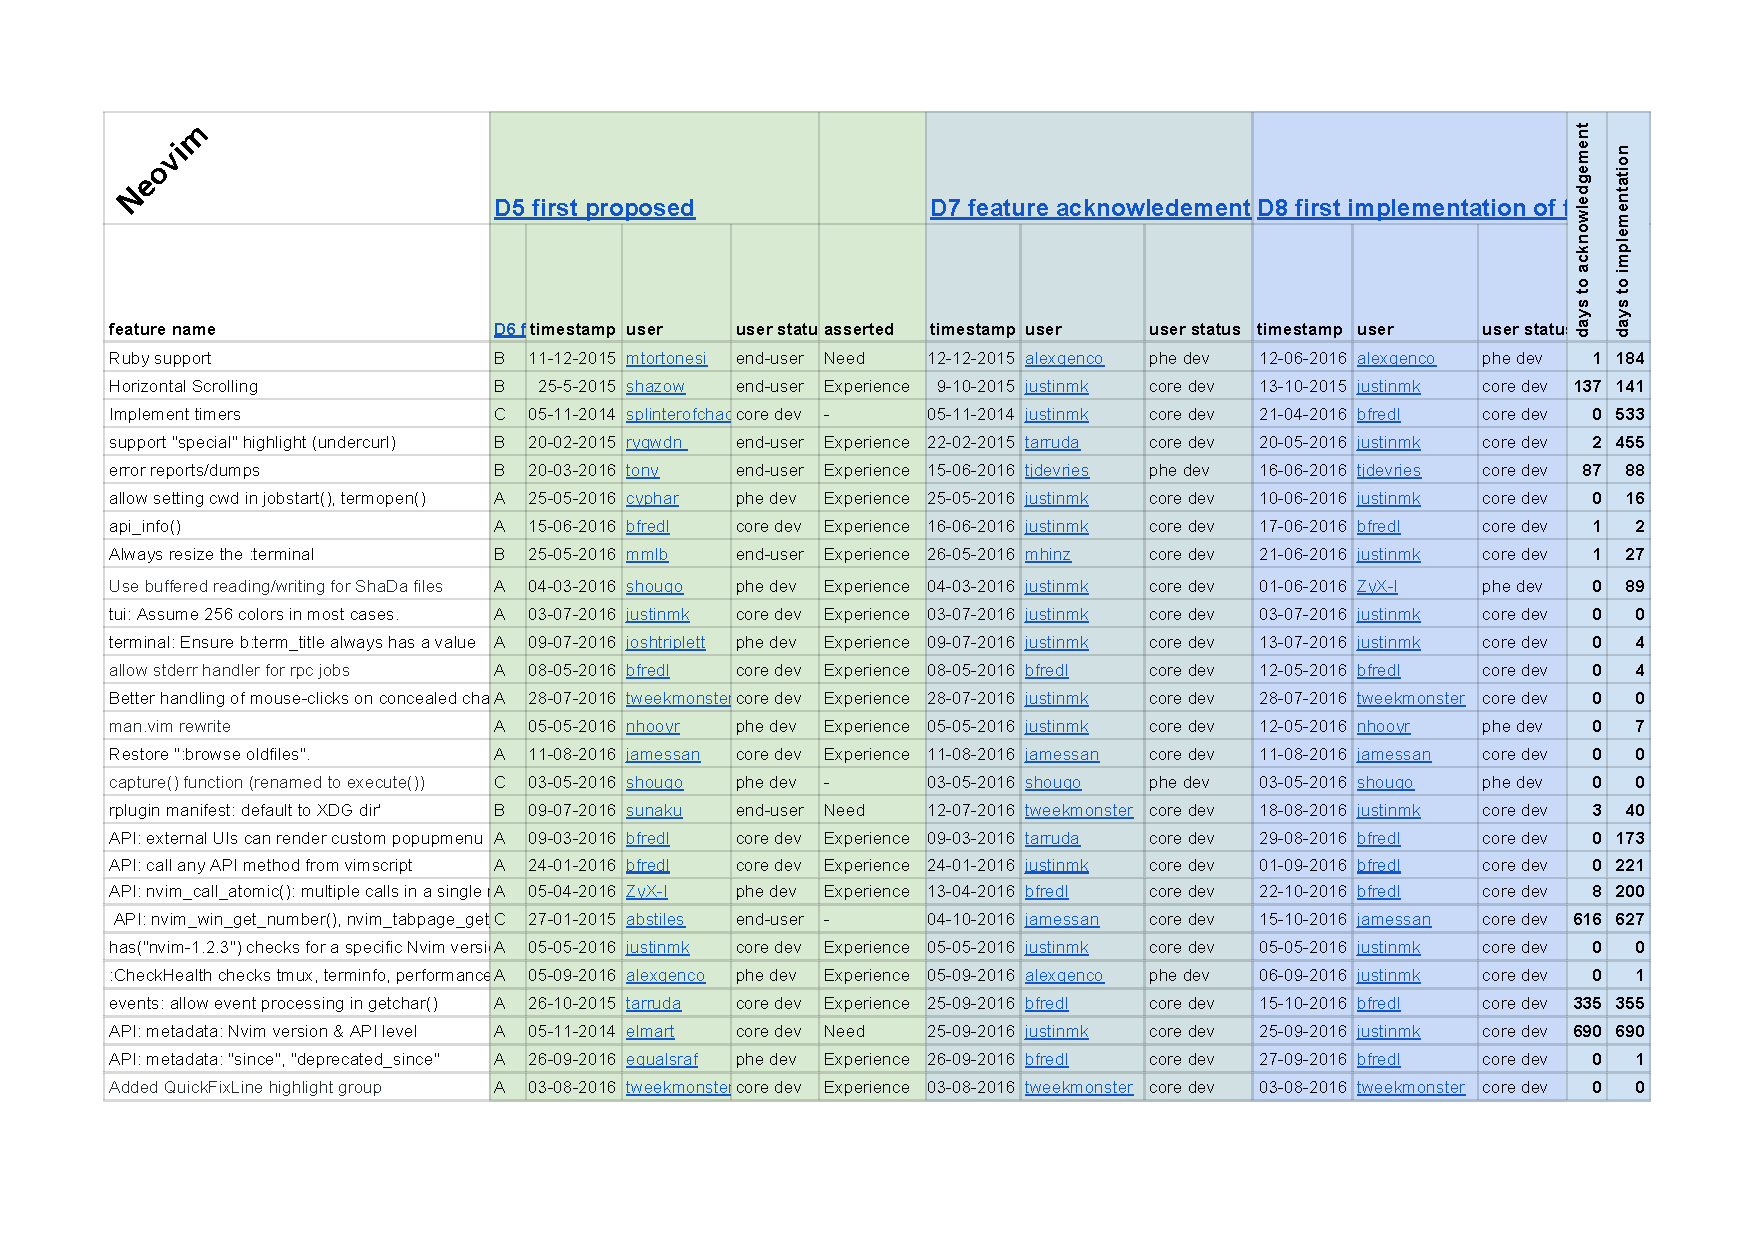
\includepdf{appendicies/detail_data_neovim}



\end{document}
